\end{document}
\newpage

\section*{Seminár 18}
\subsection*{Téma}
Algebraické výrazy a (ne)rovnice IV -- zložitejšie nerovnosti
\subsection*{Ciele}
Zoznámiť a precvičiť so študentami riešenie úloh zameraných na dokazovanie zložitejších nerovností, AG-nerovnosť
\subsection*{Úlohy a riešenia}
\begin{tcolorbox}[breakable,notitle,boxrule=0pt,colback=light-gray,colframe=light-gray]\ul 66-K-4 Dokážte, že pre všetky kladné reálne čísla $a \leq b \leq c$ platí $$(-a + b + c)\bigg( \frac{1}{a}+\frac{1}{b}+\frac{1}{c}\bigg) \geq 3.$$

\end{tcolorbox}

 \rieh  Nerovnosť vynásobíme kladným výrazom $abc$ a po roznásobení ju postupne (ekvivalentne) upravíme:
\begin{align*}
-a(bc + ac + ab) + b(bc + ac + ab) + c(bc + ac + ab) &\geq 3abc,\\
-abc - a^2c - a^2b + b^2c + abc + ab^2+ bc^2+ ac^2+ abc &\geq 3abc,\\
(b^2c - abc) + (bc^2 - abc) + (ac^2 - a^2c) + (ab^2 - a^2b) &\geq 0,\\
bc(b - a) + bc(c - a) + ac(c - a) + ab(b - a) &\geq 0.
\end{align*}
Vzhľadom na predpoklad $0 < a \leq b \leq c$ je výsledná, a teda aj pôvodná nerovnosť splnená.\\

\textbf{Iné riešenie.} Dokazovanú nerovnosť postupne upravíme, pričom využijeme známu nerovnosť $b/c + c/b = 2$, ktorá je pre kladné čísla $b, c$ ekvivalentná s nerovnosťou $(b - c)^2\geq 0$: $$(-a + b + c)\bigg( \frac{1}{a}+\frac{1}{b}+\frac{1}{c}\bigg) = 1+\bigg(\frac{b}{a}-\frac{a}{b}\bigg)+\bigg(\frac{c}{a}-\frac{a}{c}\bigg)+\bigg(\frac{b}{c}+\frac{c}{b}\bigg)\geq$$ $$
\geq 1+\frac{b^2-a^2}{ab}+\frac{c^2-a^2}{ac}+2\geq3,$$
pretože zrejme platí aj $a^2\leq b^2\leq c^2$.\\

\textbf{Iné riešenie.} Podľa predpokladov úlohy platia nerovnosti $-a + b + c \geq c$ a $\frac{1}{a}+\frac{1}{b}+\frac{1}{c}\geq \frac{2}{b}+\frac{1}{c}$.
Obe nerovnosti (s kladnými stranami) medzi sebou vynásobíme a získame tak $$(-a + b + c)\bigg(\frac{1}{a}+\frac{1}{b}+\frac{1}{c}\bigg) \geq c \bigg( \frac{2}{b}+\frac{1}{c}\bigg)=1 +\frac{2c}{b}\geq 3$$
pretože $c/b \geq 1$ podľa zadania.\\
\\
\kom Úvodná úloha slúži na opakovanie, pripomenutie naučených postupov a overenie toho, čo sa študenti doteraz naučili o nerovnostiach. Považujeme za vhodné ukázať všetky tri zmienené postupy riešenia, keďže ekvivalentné úrpavy rovníc, využívanie známych rovností aj sčítanie dvoch a viac rovností sú všetko užitočné metódy, ktoré sa oplatí mať v našej riešiteľskej zásobe.




\section{Algebra -- olympiády}
\begin{tcolorbox}[breakable,notitle,boxrule=0pt,colback=light-gray,colframe=light-gray]\ul [59-D-3-N3] V karteziánskej sústave súradníc zostrojte grafy funkcií $f: y = \lfloor x \rfloor$, $g: y = x - \lfloor x \rfloor$.\\
\end{tcolorbox}
\begin{tcolorbox}[breakable,notitle,boxrule=0pt,colback=light-gray,colframe=light-gray]\ul [59-D-3-D1] V obore reálnych čísel riešte rovnicu $\lfloor  3x-5 \rfloor = 5x - 8$. [47-C-S-1]\\
\end{tcolorbox}
\begin{tcolorbox}[breakable,notitle,boxrule=0pt,colback=light-gray,colframe=light-gray]\ul [59-D-3-D2] Nájdite všetky dvojice reálnych čísel $x, y$, pre ktoré platí $7 \lfloor x \rfloor + 2y = 117,4$ a $5x + 2 \lfloor y \rfloor = 91;9$. [47-C-I-5]\\
\end{tcolorbox}
\begin{tcolorbox}[breakable,notitle,boxrule=0pt,colback=light-gray,colframe=light-gray]\ul [59-D-3-D3] Určte všetky kladné čísla $x$, pre ktoré je medzi desiatimi číslami $\lfloor x \rfloor, \lfloor 2x \rfloor,\lfloor 3x\rfloor, \lfloor 4x \rfloor, \lfloor 5x \rfloor, \lfloor 6x\rfloor \lfloor 7x \rfloor, \lfloor 8x\rfloor, \lfloor 9x \rfloor, \lfloor 10x \rfloor$ práve deväť rôznych. [47-C-II-3]\\
\end{tcolorbox}
\begin{tcolorbox}[breakable,notitle,boxrule=0pt,colback=light-gray,colframe=light-gray]\ul
\end{tcolorbox}
Návodné a dopľňajúce úlohy:\\
\\
D1. Použitím nerovnosti $u + 1/u = 2$ $(\forall u > 0)$ dokážte, že pre ľubovoľné kladné číslo $a$
platí
a)$\frac{a^2+3}{\sqrt{a^2+2}}>2$, b)$ \frac{2a^2+1}{\sqrt{4a^2+1}}>1$.\\
{[Voľte $u =\sqrt{a^2+2}$ v prípade a), $u =\sqrt{4a^2+1}$ v prípade b) a v oboch prípadoch
využite, že $u \neq 1$.]}\\
\\
D2. Dokážte, že pre ľubovoľné kladné čísla $a, b, c, d $ platí
$$(ab + cd)  \big( \frac{1}{ac} + \frac{1}{bd}\big)\geq 4.$$
{[$L = (b/c + c/b) + (a/d + d/a) = 2 + 2 = 4$]}\\
\\
D3. Dokážte, že pre ľubovoľné čísla $a, b$ z intervalu $\langle 1, \infty)$ platí nerovnosť
$$(a^2+1)(b^2+1)-(a-1)^2(b-1)^2\geq4 $$
a zistite, kedy nastane rovnosť. {[59-C-II-2]}\\
\\
D4. Nájdite všetky reálne čísla $x$ a $y$, pre ktoré výraz $2x^2+ y^2 - 2xy + 2x + 4$ nadobúda
svoju najmenšiu hodnotu. {[65-C-I-3, časť a)]}\\
\\
Návodné a dopľňajúce úlohy:\\
\\
D2. Pre kladné reálne čísla $a, b, c$ platí $c^2+ ab = a^2+ b^2$. Dokážte, že potom platí aj $c^2+ ab \leq ac + bc$. [63-C-II-3]\\
\\
D3. Dokážte, že pre ľubovoľné nezáporné čísla $a, b, c$ platí $(a + bc)(b + ac) \geq ab(c + 1)^2$. Zistite, kedy nastane rovnosť. [58-C-S-1]\\
\\
D4. Uvažujme výraz $V (x) = (5x^4 - 4x^2+ 5)/(x^4+ 1)$.\\
a) Dokážte, že pre každé reálne číslo $x$ platí $V (x) \geq 3$.\\
b) Nájdite najväčšiu hodnotu $V (x)$. [58-C-II-1]\\
\\
D5. Dokážte, že pre ľubovoľné rôzne kladné čísla $a, b$ platí $$\frac{a+b}{2}<\frac{2(a^2+ab+b^2}{3(a+b)}<\sqrt{\frac{a^2+b^2}{2}}.$$
[58-C-I-6]\\
\\

\\
Návodné a dopľňajúce úlohy:\\
\\
N1. V obore reálnych čísel vyriešte rovnicu:\\
a) $|x| = x + 2 \ \ [x = -1]$\\
b) $|2x + 2| = x + 4 \ \ [x = -2, x = 2]$\\
c) $|x - 1| = |x| - 1 \ \ [x = 1]$\\
\\
N2. V obore reálnych čísel vyriešte sústavu rovníc:\\
a) $|x + 2| = y - 1, |y - 5| = -x \ \ [x = -3, y = 2]$\\
b) $|x - 1| = y, |x - 2| = y + 2$  [sústava nemá riešenie]\\
c) $|x| = y + 1, x = |y| + 1 \ \ [x = 1, y = 0]$\\
\\


\\
Návodné a dopľňajúce úlohy:\\
\\
N5. Nech $a, b, c, d$ sú také reálne čísla, že $a + d = b + c$. Dokážte nerovnosť $(a - b)(c - d)+ (a - c)(b - d) + (d - a)(b - c) \geq 0$. [C-54-I-1]\\
\\
N6. Pre kladné reálne čísla $a, b, c, d$ platí $a + b = c + d, ad = bc, ac + bd = 1$. Akú najväčšiu hodnotu môže mať súčet $a + b + c + d$? [C-62-I-2]\\

\begin{tcolorbox}[breakable,notitle,boxrule=0pt,colback=light-gray,colframe=light-gray]\ul 63-K-3 Pre kladné reálne čísla $a, b, c$ platí $c^2 + ab = a^2 + b^2$. Dokážte, že potom platí aj $c^2 + ab \leq ac + bc$.\\


\end{tcolorbox}

\rie Vzhľadom na podmienku $c^2 + ab = a^2 + b^2$ stačí dokázať nerovnosť $a^2 + b^2 \leq ac + bc$. Tá je ekvivalentná so vzťahom $(a^2 + b^2)^2 \leq c^2 (a + b)^2$ , ktorý vzhľadom
na danú podmienku prepíšeme na tvar $$ (a^2+ b^2)^2 \leq (a^2+
b^2 - ab)(a + b)^2.$$
Po roznásobení a zlúčení rovnakých členov zistíme, že máme dokázať nerovnosť $$0 \leq a^3b + ab^3 - 2a^2b^2= ab(a - b)^2,$$ ktorá pre kladné čísla $a, b$ zrejme platí. Vzhľadom na to, že všetky úpravy boli ekvivalentné, môžeme celý postup obrátiť. Nerovnosť je tak dokázaná.

\textbf{Iné riešenie.} Bez ujmy na všeobecnosti predpokladajme, že $0 < b \leq a$ (dané vzťahy sa výmenou čísel $a$ a $b$ nemenia). Nerovnosť $c^2 +ab \leq ac+bc$ je ekvivalentná s nerovnosťou
$(a - c)(c - b) \geq 0$, takže stačí dokázať, že $b \leq c \leq a$. Platí $$c^2 = b^2+ a^2 - ab = b^2+ a(a - b) \geq b^2,$$
teda $b \leq c$. Analogicky zistíme, že $$c^2= a^2+ b^2 - ab =a^2+ b(b - a) \leq a^2,$$
a odtiaľ $c \leq a$. Tým je dôkaz prevedený.\\
\\
\begin{tcolorbox}[breakable,notitle,boxrule=0pt,colback=light-gray,colframe=light-gray]\ul 62-D-2 Pre kladné reálne čísla $a, b, c, d$ platí
$$a + b = c + d, ad = bc, ac + bd = 1.$$
Akú najväčšiu hodnotu môže mať súčet $a + b + c + d$?

\end{tcolorbox}

\rie Najskôr ukážeme, že prvé dve rovnosti zo zadania úlohy sú splnené len vtedy, keď platí $a = c$ a súčasne $b = d$. Naozaj, vďaka tomu, že zadané čísla sú kladné (a teda rôzne od nuly), môžeme uvedené rovnosti zapísať ako
$$ a \bigg( 1+\frac{b}{a}\bigg) = c\bigg(1+\frac{d}{c}\bigg) \ \ \mathrm{a} \ \ \frac{b}{a}=\frac{d}{c}.$$
Podľa druhej rovnosti vidíme, že súčty v oboch zátvorkách z prvej rovnosti majú rovnakú kladnú hodnotu, takže sa musia rovnať prvé činitele oboch jej strán. Platí teda $a = c$, odkiaľ už vyplýva aj rovnosť $b = d$.
Keď už vieme, že platí $a = c$ a $b = d$, vystačíme ďalej len s premennými $a$ a $b$ a nájdeme najväčšiu hodnotu zadaného súčtu
$$S = a + b + c + d = 2(a + b)$$
za jedinej podmienky, totiž že kladné čísla $a, b$ spĺňajú rovnosť $a^2 + b^2 = 1$, ktorá je
vyjadrením tretej zadanej rovnosti $ac + bd = 1$ (prvé dve sú vďaka rovnostiam $a = c$ a $b = d$ zrejmé).
Všimnime si, že pre druhú mocninu (kladného) súčtu $S$ platí
$$S^2= 4(a + b)^2= 4(a^2+ b^2) + 8ab = 4 \cdot 1 + 8ab = 4(1 + 2ab),$$
takže hodnota $S$ bude najväčšia práve vtedy, keď bude najväčšia hodnota $2ab$. Zo zrejmej nerovnosti $(a - b)^2\geq 0$ po roznásobení však dostaneme
$$2ab \leq a^2+ b^2= 1,$$
pritom rovnosť $2ab = 1$ nastane práve vtedy, keď bude platiť $a = b$, čo pre kladné čísla $a, b$ spolu s podmienkou $a^2 + b^2 = 1$ vedie k jedinej vyhovujúcej dvojici $a = b = 1/\sqrt{2}$. Najväčšia hodnota výrazu $2ab$ je teda 1, takže najväčšia hodnota výrazu $S^2$ je $4(1 + 1) = 8$, a teda najväčšia hodnota $S$ je $\sqrt{8} = 2\sqrt{2}$. Dosiahne sa pre jedinú prípustnú štvoricu $a = b = c = d = 1/\sqrt{2}$.\\
\\
Návodné a dopľňajúce úlohy:\\
\\
N1. Ukážte, že nerovnosť $\frac{1}{2} (u + v) = \sqrt{uv}$ medzi aritmetickým a geometrickým priemerom
dvoch ľubovoľných nezáporných čísel $u$ a $v$ vyplýva zo zrejmej nerovnosti $(a - b)^2\geq 0$ vhodnou voľbou hodnoty $a$ a $b$. [Zvoľte $a =\sqrt{u}$ a $b =\sqrt{v}$.] Podobným obratom alebo priamym použitím uvedenej AG-nerovnosti (v niektorých prípadoch aj niekoľkonásobným) dokážte ďalšie nerovnosti $$2abc \leq a^2+ b^2c^2 \ , \ a^4+ b^4 \geq a^3b + ab^3 \, \ (1 + a + b)^2 \geq 3(a + b + ab),$$
$$\frac{a}{b^2}+\frac{b}{a^2}\geq \frac{1}{a}+\frac{1}{b}\ , \ \frac{1}{ab}+\frac{1}{cd} \geq \frac{8}{(a+b)(c+d)}\ , \ \bigg(a+\frac{1}{b} \bigg) \bigg( b+\frac{1}{c} \bigg) \bigg( c+\frac{1}{a}\bigg) \geq 8,$$
v ktorých $a, b, c, d$ označujú ľubovoľné kladné čísla.\\
\\
D1. Dokážte, že pre ľubovoľné kladné reálne čísla $a, b$ platí
$$\sqrt{ab}\leq \frac{2(a^2 +3ab+b^2)}{5(a+b)}\leq \frac{a+b}{2},$$
a pre každú z oboch nerovností zistite, kedy prechádza na rovnosť. [59-C-I-5]\\
\\
D2. Dokážte, že pre ľubovoľné rôzne kladné čísla $a, b$ platí
$$ \frac{a+b}{2}<\frac{2(a^2 +ab+b^2)}{3(a+b)}<\sqrt{\frac{a^2+b^2}{2}}.$$
[58-C-I-6]\\
\\
D3. Dokážte, že pre ľubovoľné nezáporné čísla $a, b, c$ platí $$(a + bc)(b + ac) \geq ab(c + 1)^2.$$
Zistite, kedy nastane rovnosť. [58-C-S-1]\\
\\
D5. Nech $a, b, c, d$ sú také reálne čísla, že $a + d = b + c$. Dokážte nerovnosť
$$(a - b)(c - d) + (a - c)(b - d) + (d - a)(b - c) \geq 0.$$
[54-C-I-1]\\
\\
\begin{tcolorbox}[breakable,notitle,boxrule=0pt,colback=light-gray,colframe=light-gray]\ul 61-D-4
Reálne čísla $a, b, c, d$ vyhovujú rovnici $ab + bc + cd + da = 16$.
a) Dokážte, že medzi číslami $a, b, c, d$ sa nájdu dve so súčtom najviac 4.
b) Akú najmenšiu hodnotu môže mať súčet $a^2 + b^2 + c^2 + d^2$ ?

\end{tcolorbox}

\rie a) Z rovnosti $16 = ab + bc + cd + da = (a + c)(b + d)$ vyplýva, že obidva súčty $a + c$ a $b + d$ nemôžu byť väčšie ako 4 súčasne, lebo v opačnom prípade by bol ich súčin väčší ako 16. Preto vždy aspoň jeden zo súčtov $a + c$ alebo $b + d$ má požadovanú
vlastnosť.
b) Využijeme všeobecnú rovnosť $$a^2+ b^2+ c^2+ d^2=\frac{1}{2}(a - b)^2+\frac{1}{2}(b - c)^2+\frac{1}{2}(c - d)^2+\frac{1}{2}(d - a)^2+ ab + bc + cd + da,$$
o platnosti ktorej sa ľahko presvedčíme úpravou pravej strany. Vzhľadom na nezápornosť druhých mocnín $(a-b)^2 $, $(b-c)^2$ , $(c-d)^2$ a $(d-a)^2$ dostávame pre ľavú stranu rovnosti odhad $$a^2+ b^2+ c^2+ d^2\geq ab + bc + cd + da = 16.$$
Je nájdené číslo 16 najmenšou hodnotou uvažovaných súčtov? Ináč povedané: nastane pre niektorú vyhovujúcu štvoricu v odvodenej nerovnosti rovnosť? Z nášho postupu je jasné, že musíme rozhodnúť, či pre niektorú z uvažovaných štvoríc platí $a - b = b - c = c - d = d - a = 0$, čiže $a = b = c = d$. Pre takú štvoricu má rovnosť $ab + bc + cd + da = 16$ tvar $4a^2 = 16$, čomu vyhovuje $a = \pm 2$. Pre vyhovujúce štvorice
$a = b = c = d = 2$ a $a = b = c = d = -2$ má súčet $a^2 + b^2 + c^2 + d^2$ naozaj hodnotu 16, preto ide o hľadané minimum.\\
\\
Návodné a dopľňajúce úlohy:\\

N1. Ak reálne čísla $x, y, z$ vyhovujú rovnici $x^2+y^2
= z^2$, potom aspoň jedno z čísel $|x+z|,
|x - z|$ neprevyšuje hodnotu $|y|$. Dokážte. [Keby $|x + z|, |x - z|$ boli dve (kladné) čísla
väčšie ako $|y|$, bolo by číslo $|x + z| \cdot |x - z|$ väčšie ako $|y|^2$, podľa zadania ale ide o dve
rovnaké čísla.]\\
\\
N2. Nech $x, y, z$ sú kladné reálne čísla. Ukážte, že čísla $x + y + z - xyz$ a $xy + yz + zx - 3$
nemôžu byť súčasne záporné. [60-C-II-4]\\
\\
N3. Je dané prirodzené číslo $n (n \geq 2)$ a reálne čísla $x_1, x_2, \ldots , x_n$, pre ktoré platí $x_1x_2
= x_2x_3 = \ldots = x_{n-1}x_n = x_nx_1 = 1$. Dokážte nerovnosť $x_1^2+ x_2^2+ \ldots + x_n^2\geq n$.
[55-C-I-4]\\
\\
N4. Ak reálne čísla $a, b, c, d$ vyhovujú rovnosti $a^2+ b^2= b^2+ c^2= c^2+ d^2= 1$, platí nerovnosť $ab + ac + ad + bc + bd + cd \leq 3$. Dokážte a zistite, kedy pritom nastane rovnosť. [55-C-II-2]\\
\\
N5. Dokážte, že nerovnosť $(a^2+ 1)(b^2+ 1) - (a - 1)^2
(b - 1)^2\geq  4$ platí pre ľubovoľné čísla $a, b$ z intervalu $\langle 1, \infty)$. Zistite, kedy nastane rovnosť. [59-C-II-2]\\
\\
N6. Dokážte, že nerovnosť $(a + bc)(b + ac) = ab(c + 1)^2$ platí pre ľubovoľné nezáporné čísla $a, b, c$. Zistite, kedy nastane rovnosť. [58-C-S-1]\\
\\
N7. Nerovnosti $\frac{a+b}{2}< \frac{2(a^2+ab+b^2)}{3(a+b)}<\sqrt{\frac{a^2+b^2}{2}}$  dokážte pre ľubovoľné rôzne kladné čísla $a, b$. [58-C-I-6]\\
\\
N8. Nech $a, b, c$ sú reálne čísla, ktorých súčet je 6. Dokážte, že aspoň jedno z čísel $ab + bc, bc + ca$ alebo $ca + ab$ nie je väčšie ako 8. [60-B-I-3]\\
\\
\begin{tcolorbox}[breakable,notitle,boxrule=0pt,colback=light-gray,colframe=light-gray]\ul 61-S-3
Reálne čísla $p, q, r, s$ spĺňajú rovnosti
$$p^2+ q^2+ r^2+ s^2= 4 \ \mathrm{a} pq + rs = 1.$$
Dokážte, že niektoré dve z týchto štyroch čísel sa líšia najviac o 1 a niektoré dve sa líšia
najmenej o 1.

\end{tcolorbox}

\rie Druhá zo zadaných rovníc napovedá, že by sme mali skúmať odchýlky čísel v dvojiciach $p, q$ a $r, s$. Pre súčet druhých mocnín týchto odchýlok platí
$$(p - q)^2 + (r - s)^2=  p^2+ q^2+ r^2+ s^2 - 2(pq + rs) = 4 - 2 \cdot 1 = 2.$$
Avšak ak je súčet dvoch reálnych čísel rovný číslu 2, nemôžu byť oba sčítance ani väčšie ako 1, ani menšie ako 1. Jedno z čísel $(p - q)^2 , (r - s)^2$ je teda najviac 1 a jedno je najmenej 1. To isté potom platí aj o číslach $|p - q|$ a $|r - s|$, čo sme chceli dokázať.\\
\\
\begin{tcolorbox}[breakable,notitle,boxrule=0pt,colback=light-gray,colframe=light-gray]\ul
\end{tcolorbox}

\begin{tcolorbox}[breakable,notitle,boxrule=0pt,colback=light-gray,colframe=light-gray]\ul 60-K-4
Nech $x, y, z$ sú kladné reálne čísla. Ukážte, že aspoň jedno z čísel $x + y + z - xyz$ a
$xy + yz + zx - 3$ je nezáporné.

\end{tcolorbox}

\rie Ukážeme, že ak je číslo $xy + yz + zx - 3$ záporné, je číslo $x + y + z - xyz$ kladné.
Ak $xy + yz + zx < 3$, je aspoň jedno z čísel $xy$, $yz$, $zx$ menšie ako 1, napr. $xy$. Potom $x + y + z - xyz = x + y + z(1 - xy)$ je zjavne súčet troch kladných čísel.

\textbf{Iné riešenie.} Ukážeme, že ak je číslo $x+y +z -xyz$ záporné, tak číslo $xy +yz +zx-3$ je kladné.
Predpokladajme, že $x + y + z < xyz$. Tým skôr $x < xyz$. Po skrátení kladného čísla $x$ dostaneme $yz > 1$. Podobne odvodíme odhady $xy > 1$ a $zx > 1$. Teraz ich stačí sčítať a máme $xy + yz + zx > 3$.

\textbf{Iné riešenie.} Tvrdenie úlohy dokážeme sporom. Predpokladajme, že $x + y + z < xyz$ a zároveň $xy + yz + zx < 3$. Obe tieto nerovnosti sú symetrické, preto môžeme predpokladať, že čísla $x, y, z$ sú označené tak, že $z$ je najmenšie. Z druhej nerovnosti
dostaneme, že $xy < 3$. Potom však $x + y + z < xyz < 3z$, teda $x + y < 2z$. To je však spor s tým, že číslo z je najmenšie.\\
\\
\textbf{Iné riešenie.} Aritmetický priemer $c$ čísel $a, b$ má tú vlastnosť, že sa od neho obe čísla líšia o rovnakú hodnotu $d$. Ak nahradíme premenné $a, b$ v daných nerovnostiach premennými $c, d$, zápis nerovností aj dôkaz oboch vzťahov sa zjednoduší. Položme teda $c = \frac{1}{2}(a + b)$, potom $a = c + d$ a $b = c - d$ (pričom $d =\frac{1}{2}(a - b)$, ako sa ľahko môžeme presvedčiť). Takže $a^2 + b^2 = 2(c^2 + d^2)$, $ab = c^2 - d^2$ , odkiaľ $a^2 + 3ab + b^2 = 5c^2 - d^2$.
Označme ešte písmenami $m$ a $n$ ľavú a pravú stranu prvej z dokazovaných nerovností. Potom
$$m=\sqrt{am}=\sqrt{c^2-d^2},$$
$$ n=\frac{2(a^2+3ab+b^2}{5(a+b)}=\frac{2(5c^2-d^2}{5\cdot 2c}=c-\frac{d^2}{5c}=\sqrt{\bigg(c-\frac{d^2}{5c} \bigg)^2}=\sqrt{\bigg(c-d^2\frac{2}{5}-\frac{d^2}{25c^2} \bigg)}.$$ Keďže z vyjadrenia kladnej hodnoty $m$ vidíme, že $d^2 < c^2$ , pre výraz v poslednej zátvorke pod odmocninou platí
$$1>\frac{2}{5}\geq\frac{2}{5}-\frac{d^2}{25c^2}>\frac{2}{5}-\frac{1}{25}=\frac{9}{25}>0,$$ čo znamená, že výraz pod odmocninou leží v uzavretom intervale medzi číslami $c^2 - d^2$ a $c^2$. Odtiaľ vyplýva $m \leq n \leq c$, pričom rovnosť nastane práve vtedy, keď $d = 0$, t. j. keď $a = b$.

Poznámka. Z výsledkov súťažnej úlohy vyplýva, že rozdiel medzi aritmetickým a geometrickým priemerom dvoch kladných čísel možno zdola odhadnúť nezáporným lomeným výrazom takto:
$$\frac{a+b}{2}- \sqrt{ab}\geq\frac{a+b}{2}-\frac{2(a^2+3ab+b^2}{5(a+b)}=\frac{(a-b)^2}{10(a+b)}.$$
Umocnením osamostatnenej odmocniny a ďalšími úpravami môžeme dokázať silnejší odhad rovnakého typu
$$\frac{a+b}{2}- \sqrt{ab}\geq\frac{(a-b)^2}{4(a+b)}.$$
Inú metódu dôkazov spolu s ďalšími podobnými nerovnosťami nájdete v článku J. Šimšu \textit{Dolní odhady rozdílu průměrů} v časopise Rozhledy matematicko-fyzikální 65 (1986/87), číslo 10, str. 403 -- 407.\\
\\
Návodné a dopľňajúce úlohy:\\
\\
N1. Nech $a, b, c, d$ sú také reálne čísla, že $a + d = b + c$. Dokážte nerovnosť $$(a -b)(c- d) + (a- c)(b-  d) + (d-a)(b-c)\geq 0.$$
[54-C-I-1]\\
\\
N2. Vyriešte najskôr úlohu N2 za druhou súťažnou úlohou a potom dokážte, že pre každé kladné číslo $x$ platí $x + 1/x \geq 2$. Kedy nastáva rovnosť?\\
\\
D1. Dokážte, že pre ľubovoľné rôzne kladné čísla $a, b$ platí
$$ \frac{a+b}{2}< \frac{2(a^2+ab+b^2}{3(a+b)}<\sqrt{\frac{a^2+b^2}{2}}.$$
[58-C-I-6]\\
\\
D2. Určte všetky kladné čísla $x, y, z$, pre ktoré súčasne platí
$$x +\frac{1}{y}\leq 2,  y+\frac{1}{z} \leq 2; z +\frac{1}{x} \leq 2.$$
[Sčítajte všetky tri vzťahy a ľavú stranu odhadnite pomocou nerovnosti z úlohy N2.]\\
\\

Návodné a dopľňajúce úlohy:\\
\\
N3. Nájdite všetky štvorciferné čísla $n$, ktoré majú nasledujúce tri vlastnosti: V zápise čísla $n$ sú dve rôzne cifry, každá dvakrát. Číslo $n$ je deliteľné siedmimi. Číslo, ktoré vznikne obrátením poradia cifier čísla $n$, je tiež štvorciferné a deliteľné siedmimi. [58-C-I-3]\\
\\
N4. Klárka mala na papieri napísané trojciferné číslo. Keď ho správne vynásobila deviatimi, dostala štvorciferné číslo, ktoré začínalo rovnakou číslicou ako pôvodné číslo, prostredné dve číslice sa rovnali a posledná číslica bola súčtom číslic pôvodného čísla.
Ktoré štvorciferné číslo mohla Klárka dostať? [57-C-I-6]\\
\\

\\
Návodné a dopľňajúce úlohy:\\
\\
N1. Pre $a, b \in \RR$ dokážte $$a^4+ b^4\geq a^3b + b^3a.$$
[Upravte na tvar $(a^3 -  b^3)(a -  b)  \geq 0$.]\\
\\
D1. Dokážte, že pre každé tri reálne čísla $x, y, z$, ktoré spĺňajú nerovnosti $0 < x < y < z < 1$, platí nerovnosť $$x^2+ y^2+ z^2< xy + yz + zx + z-x.$$
[48-C-II-4]\\
\\
D2. Dokážte, že pre ľubovoľné kladné čísla $a, b$ a $c$ platí nerovnosť
$$\bigg( a +\frac{1}{b}\bigg)\bigg( b +\frac{1}{c}\bigg)\bigg( c +\frac{1}{a}\bigg)\geq 8.$$
[55-B-S-1]\\
\\
D3. Ak reálne čísla $a, b, c, d$ spĺňajú rovnosti
$$a^2+ b^2= b^2+ c^2= c^2+ d^2= 1,$$
platí nerovnosť
$$ab + ac + ad + bc + bd + cd \leq 3.$$
Dokážte a zistite, kedy nastane rovnosť. [55-C-II-2]\\
\\

\begin{tcolorbox}[breakable,notitle,boxrule=0pt,colback=light-gray,colframe=light-gray]\ul 58-K-1
 Uvažujme výraz $$V(x) =\frac{5x^4 - 4x^2 + 5}{x^4 + 1}.$$

a) Dokážte, že pre každé reálne číslo $x$platí $V (x) \geq 3$.

b) Nájdite najväčšiu hodnotu $V (x)$.

\end{tcolorbox}

\rie  Výraz $V$ je zrejme definovaný pre všetky reálne čísla $x$.

a) Keďže $x^4 +1 > 0$ pre každé $x$, nerovnosť $V (x) \geq 3$ je ekvivalentná s nerovnosťou $5x^4 - 4x^2 + 5 \geq 3(x^4 + 1)$, čiže $2x^4 - 4x^2 + 2 \geq 0$. Výraz na ľavej strane je rovný $2(x^2 - 1)^2$, takže je nezáporný pre každé $x$.

b) Využime nasledujúcu úpravu:
$$V (x) =\frac{5x^4 - 4x^2 + 5}{x^4 + 1}=\frac{5(x^4 +1)}{x^4 + 1}-\frac{4x^2}{x^4 + 1}=5-\frac{4x^2}{x^4 + 1}.$$
Keďže zlomok
$$\frac{4x^2}{x^4 + 1}$$
je vďaka párnym mocninám premennej $x$ pre ľubovoľné reálne číslo $x$ nezáporný, nadobúda výraz $V$ svoju najväčšiu hodnotu $V_{max}$ práve vtedy, keď
$$\frac{4x^2}{x^4 + 1}=0$$
teda práve vtedy, keď $x = 0$. Dostávame tak $V_{max} = V (0) = 5$.\\
\\

Návodné a dopľňajúce úlohy:\\
\\
\\
\\
N2. Nováková, Vašková a Sudková vyhrali štafetu a okrem diplomov dostali aj bonboniéru, ktorú hneď po pretekoch zjedli. Keby zjedla Petra o 3 bonbóny viac, zjedla by ich práve toľko, koľko Miška s Janou dokopy. A keby si Jana pochutnala ešte na siedmich bonbónoch, tiež by ich mala toľko, ako druhé dve spolu. Ešte vieme, že počet bonbónov, ktoré zjedla Vašková, je deliteľný tromi a že Sudková si pochutila na siedmich bonbónoch. Ako sa volali dievčatá? Koľko bonbónov zjedla každá z nich? [56-Z9-II-3]\\
\\

Návodné a dopľňajúce úlohy:
\\
\begin{tcolorbox}[breakable,notitle,boxrule=0pt,colback=light-gray,colframe=light-gray]\ul 57-K-2
Klárka urobila chybu pri písomnom násobení dvoch dvojciferných čísel, a tak jej vyšlo číslo o 400 menšie, ako bol správny výsledok. Pre kontrolu vydelila číslo, ktoré dostala, menším z násobených čísel. Tentoraz počítala správne a vyšiel jej neúplný podiel 67 a zvyšok 56. Ktoré čísla Klárka násobila?

\end{tcolorbox}

\rie Označme $x$ menšie a $y$ väčšie z násobených čísel. Podľa zadania platí $xy - 400 = 67x + 56$, čiže
$$x(y - 67) = 456. (1)$$
Číslo $x$ je teda dvojciferný deliteľ čísla $456 = 2^3\cdot 3 \cdot 19$. Zo zadania navyše vyplýva,
že číslo $x$ je väčšie ako príslušný zvyšok 56. Najmenšie také $x$ je $x = 3 \cdot 19 = 57$. Pre
každý ďalší taký deliteľ platí $x \geq 4 \cdot 19 = 76$ a $y - 67 \leq 2 \cdot 3 = 6$, takže $y \leq 73 < x$, čo odporuje zvolenému označeniu $x < y$. Teda $x = 57$ a $y = 75$. Ľahko overíme, že tieto čísla vyhovujú zadaniu úlohy.

Záver. Klárka násobila čísla 57 a 75.\\
\\

\newpage
\section{Teória čísel}


\\
Návodné a dopľňajúce úlohy:\\
\\

\\
D2. Dokážte, že pre ľubovoľné celé čísla $n$ a $k$ väčšie ako 1 je číslo $n^{k+2} - n^k$ deliteľné
dvanástimi. [59-C-II-1]\\
\\
D3. Dokážte, že výrazy $23x + y$, $19x + 3y$ sú deliteľné číslom 50 pre rovnaké dvojice prirodzených čísel $x$, $y$. [60-C-I-2]\\
\\
D4. Určte všetky celé čísla $n$, pre ktoré $2n^3 - 3n^2+ n + 3$ je prvočíslo. [62-C-I-5]\\
\\
D5. Dokážte, že pre každé nepárne prirodzené číslo $n$ je súčet $n^4+ 2n^2+ 2 013$ deliteľný číslom 96. [63-C-I-5]\\
\\



\\
Návodné a dopľňajúce úlohy:\\
\\
N1. Určte všetky prirodzené čísla $a$ a $b$, pre ktoré je rozdiel $a^2 - b^2$ druhou mocninou
niektorého prvočísla. [$a = (p^2+ 1)/2$ a $b = (p^2 - 1)/2$, pričom $p$ je ľubovoľné nepárne prvočíslo.]\\
\\
D1. Nájdite všetky dvojice nezáporných celých čísel $a$, $b$, pre ktoré platí $a^2+b+2 = a+b^2$. [59-C-S-3]\\
\\


\\
Za úplné riešenie dajte 6 bodov, z toho 3 body za popis vyhrávajúcej Barborinej stratégie v prípade, keď začína Adam, a 3 body za popis vyhrávajúcej Adamovej stratégie v prípade, keď začína Barbora. Obe opísané vyhrávajúce stratégie nie sú samozrejme jediné možné, napríklad Adam môže založiť svoju stratégiu na deliteľnosti jedenástimi namiesto tromi, keď svojimi ťahmi dosiahne rovnosť $c = d$ a nerovnosť a $6= b$.\\
\\

Prácnejšou úlohou by bolo nájsť najmenšie číslo $n$, pre ktoré za desatinnou čiarkou iracionálneho čísla $\sqrt{n}$ sú dve osmičky, či dve sedmičky a pod.\\
\\
Návodné a dopľňajúce úlohy:\\

N1. Ak nie je prirodzené číslo $n$ druhou mocninou iného prirodzeného čísla, dokážte, že $\sqrt{n}$ je číslo iracionálne.\\
\\
N2. Nájdite pomocou kalkulačky najmenšie prirodzené číslo $n$ také, že v zápise iracionálneho čísla $\sqrt{n}$ nasleduje bezprostredne za desatinnou čiarkou deviatka. [$\sqrt{35} = 5,916 079 \ldots$]\\
\\
N3. Nájdite všetky prirodzené čísla $n$ také, že v zápise iracionálneho čísla $\sqrt{n}$ nasleduje bezprostredne za desatinnou čiarkou deviatka.\\
\\
N4. Nájdite najmenšie prirodzené číslo $n$ také, že v zápise iracionálneho čísla $\sqrt{n}$ nasledujú bezprostredne za desatinnou čiarkou dve nuly. [$\sqrt{2 501} = 50,009 999 \ldots$ ]\\
\\
N5. Nájdite najmenšie prirodzené číslo $n$ také, že v zápise iracionálneho čísla $\sqrt{n}$ nasledujú bezprostredne za desatinnou čiarkou dve rovnaké cifry. [Na kalkulačke $\sqrt{43}= 6,557 438\ldots$]\\
\\

Hľadané číslo je n = 2 015.\\
\\
\
\\
\begin{tcolorbox}[breakable,notitle,boxrule=0pt,colback=light-gray,colframe=light-gray]\ul [64-K-4]
Hovoríme, že kladné reálne číslo je copaté, ak nie je prirodzené a vo svojom dekadickom zápise obsahuje za desatinnou čiarkou iba konečne veľa nenulových cifier.

a) Nájdite dve copaté čísla $a, b$ také, že $a \cdot b =2015$.

b) Rozhodnite, či existujú tri copaté čísla $a, b, c$ také, že čísla $a \cdot b$, $b \cdot c$ a $c \cdot a$ sú
všetky prirodzené.

\end{tcolorbox}

\rieh a) Takých dvojíc copatých čísel je nekonečne veľa. Je to napr. dvojica $$a = 2 015 \cdot \frac{5}{2}=5037,5, \ \ \ b =\frac{2}{}5= 0,4.$$

Podobne vyhovuje každá z nekonečne veľa dvojíc
$$a = 2 015 \cdot \frac{5^m}{2^n},\ \ \  b =\frac{2^n}{5^m},$$
pričom $m$ a $n$ sú ľubovoľné prirodzené čísla. Uvedené číslo $a$ má $n$ desatinných miest, číslo $b$ ich má $m$.

b) Taká trojica copatých čísel neexistuje. Každé copaté číslo, ktoré má za desatinnou čiarkou poslednú nenulovú cifru na $k$-tom mieste, t. j. na mieste rádu $10^{-k}$, môžeme pre vhodné prirodzené číslo s zapísať ako $s \cdot 10^{-k} (k \geq 1)$. Pritom $s$ nie je deliteľné desiatimi, môže teda byť deliteľné iba  jedným z prvočísel 2 alebo 5, a to ľubovoľnou jeho mocninou.

Súčinom dvoch copatých čísel $a = s/10^k$ a $b = t/10^l$ dostaneme prirodzené číslo iba vtedy, keď je súčin $st$ deliteľný $10^{k+l}$ , čiže keď jedno z čísel $s, t$ je deliteľné $2^k+l$ a druhé $5^k+l$, pričom $k + l = 2$. Ak sú teda $a = s/10^k$, $b = t/10^l$, $c = u/10^m$ ľubovoľné copaté čísla také, že súčiny $a \cdot b$ a $a \cdot c$ sú prirodzené čísla, je z predchádzajúcej úvahy zrejmé, že obe čísla $t$ aj $u$ musia byť buď obe nepárne a deliteľné piatimi, alebo naopak obe párne a nedeliteľné piatimi, takže ich súčin tu nemôže byť deliteľný desiatimi, teda súčin $bc = tu/10^{l+m}$ nemôže byť celý.\\
\\
Návodné a dopľňajúce úlohy:\\

N1. Určte všetky prvočísla $p, q$, pre ktoré platí $p + q = 14$.\\
\\

\\
N3. Číslo $n$ je súčinom dvoch prvočísel. Ak zväčšíme jedno z nich o 1 a druhé o 1 zmenšíme, ich súčin ostane nezmenený. Určte číslo $n$. [Výsledok: $n = 6$.]\\
\\

Návodné a dopľňajúce úlohy:\\

N5. Určte všetky celé čísla $n$, pre ktoré je $2n^3 - 3n^2+ n + 3$ prvočíslo. [C-62-I-5]\\
\\

Návodné a dopľňajúce úlohy:\\
N1. a) Dokážte, že pre každé prirodzené číslo $m$ je rozdiel $m^6 - m^2$ deliteľný číslom 60.\\
b) Určte všetky prirodzené čísla m, pre ktoré je rozdiel $m^6 - m^2$ deliteľný číslom 120. [C-55-I-1] \\
\\

\\
D1. Dokážte, že pre ľubovoľné celé čísla $n$ a $k$ väčšie ako 1 je číslo $n^{k+2} - n^k$ deliteľné dvanástimi. [C-59-II-1]\\
\\
Návodné a dopľňajúce úlohy:\\
\\
N2. Dokážte, že pre ľubovoľné prirodzené čísla $a, b$ platí vzťah $[a, b] \cdot (a, b) = ab$. [Podľa úvahy o počtoch zastúpení každého prvočísla v číslach $a, b, (a, b) a [a, b]$ stačí vysvetliť, prečo pre akékoľvek čísla $\alpha, \beta$ platí rovnosť $\min\{\alpha, \beta\} + \max \{\alpha, \beta\} = \alpha + \beta$. K tomu stačí rozlíšiť prípady $\alpha < \beta$, $\alpha = \beta$ a $\alpha > \beta$. Iné riešenie: Nech $d = (a, b)$, potom $a = xd$, $b = yd$ pre nesúdeliteľné $x$ a $y$, odtiaľ vyplýva $[a, b] = xyd$, takže oba súčiny $[a, b] \cdot (a, b)$ a $ab$ sa rovnajú číslu $xyd^2$.]\\
\\
N5. Pre ľubovoľné prirodzené čísla $a, b$ dokážte nerovnosť $a \cdot (a, b) + b \cdot [a, b] \geq 2ab$. Zistite tiež, kedy v tejto nerovnosti nastane rovnosť. [60-C-I-5]\\
\\

Návodné a dopľňajúce úlohy:\\
\\

\\

\\

\\
Návodné a dopľňajúce úlohy:\\
\\
N4. Dokážte, že pre kladné reálne čísla $a, b$ platí
$$4ab \leq (a + b)^2 \leq 2(a^2+ b^2).$$
[Obe nerovnosti sa dajú priamočiaro ukázať z toho, že štvorec reálneho čísla je nezáporný.]\\
\\
D1. Nájdite všetky trojice prirodzených čísel $a, b, c$, pre ktoré súčasne platí $[ab, c] = 2^8$, $[bc, a] = 2^9$, $[ca, b] = 2^11$. [50-C-S-1]\\
\\
D4. Dokážte, že pre ľubovoľné rôzne kladné čísla $a, b$ platí
$$\frac{a + b}{2}<\frac{2(a^2+ ab + b^2)}{3(a + b)}< \sqrt{\frac{a^2 + b^2}{2}}.$$
\\

\\

\\

Návodné a dopľňajúce úlohy:\\
\\
N3. K prirodzenému číslu $m$ zapísanému rovnakými ciframi sme prečítali štvorciferné prirodzené číslo $n$. Získali sme štvorciferné číslo s opačným poradím cifier, než má
číslo $n$. Určte všetky také dvojice čísel $m$ a $n$. [52-C-I-5]\\
\\

Návodné a dopľňajúce úlohy:\\
\\
N1. Ukážte, že z ľubovoľných $n$ prirodzených čísel možno vybrať niekoľko (napríklad aj jedno) tak, že ich súčet je deliteľný číslom $n$. [Uvažujte čísla $a_1, a_1 +a_2, \ldots , a_1 + \cdots  + a_n$ a ich zvyšky po delení $n$.]\\
\\
N2. Zistite, pre ktoré prirodzené čísla $n (n \geq 2)$ je možné z množiny $\{1; 2; \ldots; n -1\}$ vybrať aspoň dve navzájom rôzne párne čísla tak, aby ich súčet bol deliteľný číslom $n$. [54-C-I-2]\\
\\
D1. Určte počet všetkých trojíc navzájom rôznych  rojciferných prirodzených čísel, ktorých súčet je deliteľný každým z troch sčítaných čísel. [55-C-I-3]\\
\\
\begin{tcolorbox}[breakable,notitle,boxrule=0pt,colback=light-gray,colframe=light-gray]\ul [58-K-3]
Z množiny $\{1, 2, 3, \ldots , 99\}$ je vybraných niekoľko rôznych čísel tak, že súčet žiadnych troch z nich nie je násobkom deviatich.

a) Dokážte, že medzi vybranými číslami sú najviac štyri deliteľné tromi.
b) Ukážte, že vybraných čísel môže byť 26.

\end{tcolorbox}

\rieh Podľa zvyškov po delení deviatimi rozdelíme všetkých 99 uvažovaných čísel do deviatich jedenásťprvkových tried $T_0, T_1 , \ldots, T_8$ (do triedy $T_i$ patria všetky čísla so zvyškom $i$):
\begin{center}
\begin{align*}
T_0 &= \{9, 18, 27, \ldots , 99\},\\
T_1 &= \{1, 10, 19, \ldots, 91\},\\
T_2 &= \{2, 11, 20, \ldots , 92\},\\
\vdots\\
T_8 &= \{8, 17, 26, \ldots , 98\}.
\end{align*}
\end{center}

a) Našou úlohou je dokázať, že v $T_0\cup T_3 \cup T_6$ ležia najviac štyri vybrané čísla. Z každej z tried $T_0, T_3, T_6$ môžu pochádzať najviac dve z vybraných čísel (súčet ľubovoľných troch čísel z jednej takej triedy už totiž deliteľný deviatimi je). Keďže súčet ľubovoľných troch čísel, ktoré po jednom ležia v triedach $T_0, T_3 a T_6$, je deviatimi deliteľný, aspoň jedna z týchto tried žiadne vybrané číslo neobsahuje. Z oboch vyslovených záverov vyplýva dokazované tvrdenie: vybraných čísel deliteľných tromi je totiž najviac $2 + 2 + 0 = 4$.

b) Ukážeme, že vyhovujúci výber môže obsahovať 26 čísel. Vyberieme po dvoch číslach z $T_0, T_3$ a po 11 číslach (teda všetky čísla) z $T_1$ a $T_2$. Dostaneme tak celkom $2 \cdot 2 + 2 \cdot 11 = 26$ čísel; pritom súčet ľubovoľných troch z nich dáva po delení deviatimi zvyšok aspoň $0 + 0 + 1 = 1$, najviac však $2 + 3 + 3 = 8$, takže deviatimi deliteľný byť
nemôže.\\
\\

Návodné a dopľňajúce úlohy:\\
\\

D1. Nájdite všetky trojice prirodzených čísel $a, b, c$, pre ktoré súčasne platí
$$ n(ab,c) = 2^8, \ \ \  n(bc,a) = 2^9, \ \ \ n(ca,b) = 2^11,$$
pričom $n(x, y)$ označuje najmenší spoločný násobok prirodzených čísel $x, y$. [50-C-S-1]\\
\\
D2. Pre koľko usporiadaných trojíc prirodzených čísel $x, y, z$ platí $xyz = 1 000 000$? [Návod: $1 000 000 = 2^6\cdot5^6$. Položme $x = 2^a5^p$, $y = 2^b5^q$, $z = 2^c5^r$ a preskúmajme všetky možnosti pre $a + b + c = 6$ a pre $p + q + r = 6$. Nakoniec zistíme hľadaný počet: $28\cdot28 = 784$.]\\
\\

\section{Všeličo}
\begin{tcolorbox}[breakable,notitle,boxrule=0pt,colback=light-gray,colframe=light-gray]\ul [66-D-6]\\
\\

\ul [65-D-2]
Určte, koľkými spôsobmi možno k jednotlivým vrcholom kocky $ABCDEFGH$ pripísať čísla 1, 3, 3, 3, 4, 4, 4, 4 tak, aby súčin čísel pripísaných ľubovoľným trom vrcholom každej zo stien kocky bol párny.

\end{tcolorbox}

\rieh Pre kontrolu dotyčnej podmienky stačí vedieť len to, ktorým vrcholom kocky $ABCDEFGH$ sú pripísané čísla nepárne a ktorým čísla párne. Zaveďme preto znaky $N$ a $P$ pre všetky nepárne, resp. párne čísla a riešme najskôr otázku, koľkými vyhovujúcimi spôsobmi môžeme pripísať k vrcholom kocky $ABCDEFGH$ štyri $N$ a štyri $P$ (práve toľko ich totiž je medzi zadanými číslami 1, 3, 3, 3, 4, 4, 4, 4).

Uvedomme si, čo podmienka úlohy hovorí o počte znakov $N$ pripísaných vrcholom jednej a tej istej steny kocky: počet týchto $N$ je nanajvýš 2 (súčin troch pripísaných $N$ by bol totiž nepárny, teda v rozpore s danou podmienkou). Keď však danú stenu kocky zvážime súčasne so stenou s ňou rovnobežnou (t. j. stenou protiľahlou), pri ktorej vrcholoch sú tiež nanajvýš dve $N$, a zohľadníme pritom, že pri ôsmich vrcholoch týchto dvoch stien (teda pri všetkých ôsmich vrcholoch kocky) sú (všetky) štyri $N$, dôjdeme 1k záveru, že pri vrcholoch každej steny sú práve dve $N$ (a teda aj dve $P$). Naopak, každé také pripísanie štyroch $N$ a štyroch $P$ zrejme vyhovuje požiadavkám úlohy.

Stojíme tak pred úlohou určiť počet tých pripísaní štyroch $N$ a štyroch $P$ vrcholom kocky $ABCDEFGH$, pri ktorých sú dve $N$ a dve $P$ pri vrcholoch každej steny. Rozdelíme ich na dve skupiny podľa toho, či existuje stena, na ktorej sú obe $N$
priradené vrcholom susedným (na kocke tak vznikne aspoň jedna hrana ”$NN$“), alebo naopak vo všetkých stenách sú obe $N$ priradené vrcholom protiľahlým (všetky hrany kocky potom budú
”$N$P“). Po jednom reprezentantovi oboch skupín vidíme na obr. 1 -- pre lepší prehľad bez označenia vrcholov kocky písmenami. Ľahko overíme (výklad tu vynecháme), že znaky v krúžku pri reprezentantoch oboch skupín už jednoznačne určujú znaky pri všetkých ostatných vrcholoch kocky.
\begin{center}
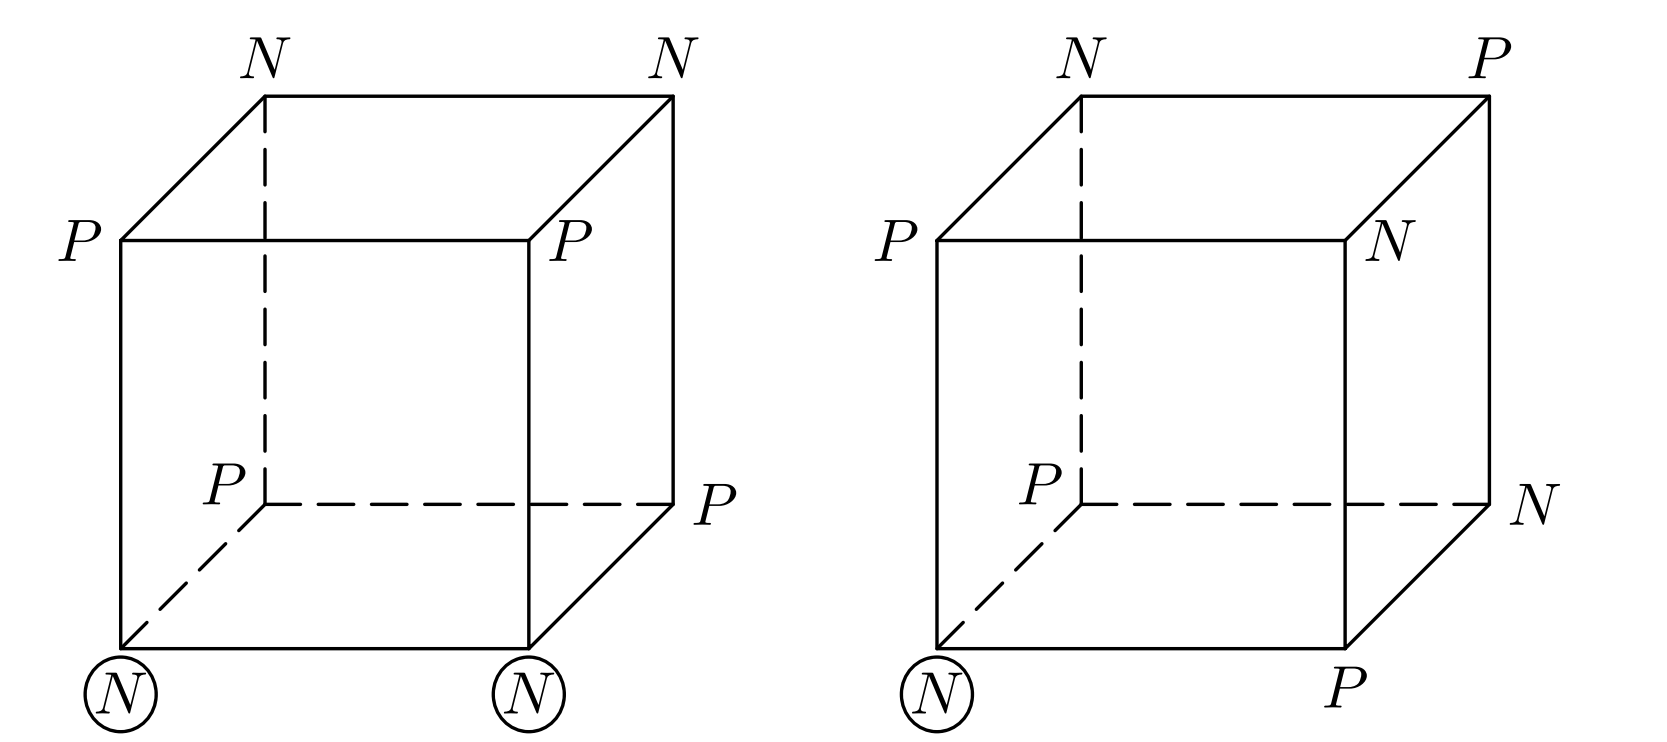
\includegraphics[width=0.6\textwidth]{NPkocka}
\end{center}

Teraz už ľahko usúdime, že v prvej skupine je práve šesť priradení -- jednou hranou ”$NN$“ je totiž, ako vieme, celé vyhovujúce priradenie určené a má práve dve hrany ”$NN$“, ktoré sú pritom rovnobežné a neležia v jednej stene; takých dvojíc hrán je pre kocku $ABCDEFGH$ práve šesť. Naproti tomu v druhej skupine sú iba dve rzne priradenia -- pretože sa jedná o priradenie bez hrany ”$NN$“; znakom $P$ alebo $N$ pri vrchole $A$ danej kocky sú totiž, ako vieme, určené znaky pri všetkých ďalších jej vrcholoch. Existuje tak spolu $6 + 2 = 8$ vyhovujúcich priradení štyroch $N$ a štyroch $P$ vrcholom kocky $ABCDEFGH$.

V ďalšej, jednoduchšej časti nášho postupu určíme, koľkými spôsobmi môžeme štyri $N$ a štyri $P$ (pevne pripísané vrcholom kocky) zameniť konkrétnymi číslami 1, 3, 3, 3, 4, 4, 4, 4. Máme zrejme práve štyri možnosti pre výber toho $N$, ktoré zameníme číslom 1; potom už zvyšné tri $N$ musíme zameniť číslom 3, rovnako ako všetky štyri $P$ číslom 4. Počet spôsobov zámen znakov $N$ a $P$ danými číslami je tak rovný 4.

Nakoniec uplatníme jednoduché kombinatorické pravidlo súčinu: keďže existuje osem vyhovujúcich pripísaní znakov $N$ a $P$ k vrcholom danej kocky a pri každom z nich možno štyrmi spôsobmi zameniť znaky $N$ a $P$ danými číslami, je hľadaný počet vyhovujúcich pripísaní daných čísel vrcholom danej kocky rovný $8 \cdot 4 = 32$.\\
\\
Návodné a dopľňajúce úlohy:\\
\\
N1. Koľkými spôsobmi možno vrcholom štvorca $ABCD$ a jeho stredu $P$ pripísať čísla 1, 2, 3, 4, 5 tak, aby boli napospol nepárne súčty čísel pri každej jeho strane aj oboch uhlopriečkach? Dokážete tento počet určiť bez toho, aby ste vypísali všetky možnosti a potom ich spočítali? [24 spôsobov. Najskôr pripíšte daným piatim bodom tri znaky $N$ a dva znaky $P$ pre nepárne, resp. párne čísla -- to možno spraviť práve
dvoma vyhovujúcimi spôsobmi. Potom uvážte, že znaky $N$ možno zameniť danými číslami šiestimi spôsobmi a znaky $P$ dvoma spôsobmi.]\\
\\
D1. Určte, koľkými spôsobmi možno vrcholom pravidelného 9-uholníka $ABCDEFGHI$ priradiť čísla z množiny $\{17, 27, 37, 47, 57, 67, 77, 87, 97\}$ tak, aby každé z nich bolo priradené inému vrcholu a aby súčet čísel priradených každým trom susedným vrcholom bol deliteľný tromi. [61-B-II-2]\\
\\
\begin{tcolorbox}[breakable,notitle,boxrule=0pt,colback=light-gray,colframe=light-gray]\ul [65-D-5] Máme kartičky s číslami $5, 6, 7, \ldots, 55$ (na každej kartičke je jedno číslo). Koľko najviac kartičiek môžeme vybrať tak, aby súčet čísel na žiadnych dvoch vybraných kartičkách nebol palindróm? (Palindróm je číslo, ktoré je rovnaké pri čítaní zľava doprava i sprava doľava.)

\end{tcolorbox}

\rieh Aby sme sa mohli stručnejšie vyjadrovať, budeme vyberať priamo \textit{čísla}, a nie kartičky.

Všimnime si najskôr, že pre súčet s ľubovoľných dvoch daných čísel platí $11 = 5 + 6 \leq  s \leq 55 + 54 = 109$. Medzi číslami od 11 po 109 sú palindrómy práve všetky násobky 11 a navyše aj číslo 101. Uvedomme si teraz, že deliteľnosť súčtu dvoch čísel daným číslom $d$ (nám pôjde o hodnotu $d = 11$) závisí iba na zvyškoch oboch sčítaných čísel po delení dotyčným $d$. Toto užitočné pravidlo uplatníme tak, že všetky dané čísla
od 5 po 55 rozdelíme do skupín podľa ich zvyškov po delení číslom 11 a tieto skupiny zapíšeme do riadkov tak, aby súčet dvoch čísel z rôznych skupín na rovnakom riadku bol deliteľný číslom 11; o význame zátvoriek na konci každého riadku budeme hovoriť vzápätí.
\begin{center}
\begin{align*}
\{5, 16, 27, 38, 49\}&, \ \ \ \{6, 17, 28, 39, 50\} &\text{(5 čísel)},\\
\{7, 18, 29, 40, 51\}&, \ \ \ \{15, 26, 37, 48\}  &\text{(5 čísel)},\\
\{8, 19, 30, 41, 52\}&, \ \ \ \{14, 25, 36, 47\} &\text{(5 čísel)},\\
\{9, 20, 31, 42, 53\}&, \ \ \ \{13, 24, 35, 46\}  &\text{(5 čísel)},\\
\{10, 21, 32, 43, 54\}&, \ \ \ \{12, 23, 34, 45\} &\text{(5 čísel)}\\
\{11, 22, 33,& 44, 55\} \ \ &\text{(1 číslo)}.
\end{align*}
\end{center}

Na koniec každého riadku sme pripísali maximálny počet na ňom zapísaných čísel, ktoré môžeme súčasne vybrať bez toho, aby súčet dvoch z nich bol násobkom čísla 11. Napríklad v treťom riadku máme päticu čísel so zvyškom 8 a štvoricu čísel so zvyškom 3. Je jasné, že nemôžeme súčasne vybrať po čísle z oboch týchto skupín (ich súčet by bol násobkom 11), môžeme však vybrať súčasne všetkých päť čísel z pätice (súčet každých dvoch z nich bude po delení 11 dávať taký istý zvyšok ako súčet 8 + 8, teda zvyšok 5). Dodajme ešte, že uvedená schéma šiestich riadkov má pre nás ešte jednu obrovskú výhodu: súčet žiadnych dvoch čísel z rôznych riadkov nie je násobkom 11 (tým totiž nie
je ani súčet ich dvoch zvyškov).

Z uvedeného rozdelenia všetkých daných čísel do šiestich riadkov vyplýva, že vyhovujúcim spôsobom nemôžeme vybrať viac ako $5 \cdot 5 + 1 = 26$ čísel. Keby sme však vybrali 26 čísel, muselo by medzi nimi byť aj jedno z čísel 49 alebo 50 a z ďalších štyroch riadkov postupne čísla 51, 52, 53 a 54 -- potom by sme ale dostali palindróm 49 + 52 alebo 50 + 51. A tak sa nedá vybrať viac ako 25 čísel, pritom výber 25 čísel možný je: z prvých piatich riadkov vyberieme napríklad všetky čísla z ľavých skupín s výnimkou čísla 52 a k tomu jedno číslo (napríklad 11) z posledného riadku. Potom súčet žiadnych dvoch vybraných čísel nebude deliteľný 11 (vďaka zaradeniu čísel do skupín), ani rovný poslednému ”kritickému“ číslu, palindrómu 101 (preto sme pri voľbe čísla 49 vylúčili 52).\\
\textit{Odpoveď}. Najväčší možný počet kartičiek, ktoré môžeme požadovaným spôsobom vybrať, je rovný číslu 25.
\textbf{Iné riešenie}. Medzi vybranými číslami môžu byť
\begin{itemize}
\item iba jedno číslo z pätice (11, 22, 33, 44, 55);
\item nanajvýš jedno číslo z každej z 20 nasledujúcich dvojíc (5, 6), (7, 15), (8, 14), (9, 13), (10, 12), (16, 17), (18, 26), (19, 25), (20, 24), (21, 23), (27, 28), (29, 37), (30, 36), (31, 35), (32, 34), (38, 39), (40, 48), (41, 47), (42, 46) a (43, 45); \footnote{Tieto dvojice so súčtami deliteľnými číslom 11 sme vytvorili postupne zo zvyšných čísel tak, že sme k najmenšiemu doposiaľ nezapísanému číslu sme pripojili ďalšie najmenšie doposiaľ nezapísané číslo, ktoré ”dopľňa“ prvé číslo na nejaký násobok 11. Takému postupu sa najmä v matematickej
informatike hovorí pažravý \textit{algoritmus}.}
\item nanajvýš dve čísla zo štvorice (49, 50, 51, 52) (pretože súčty 49 + 50, 50 + 51 a 49 + 52 sú palindrómy);
\item obe zvyšné čísla 53 a 54.
\end{itemize}

Preto sa nedá požadovaným spôsobom vybrať viac ako 1 + 20 + 2 + 2 = 25 čísel. Vyhovujúci výber 25 čísel je možný: jedno číslo z pätice násobkov 11, menšie z dvoch čísel z každej z 20 dvojíc, čísla 49 a 51 zo štvorice a napokon obe čísla 53 a 54. Je však nutné vysvetliť, prečo súčet žiadnych dvoch vybraných čísel nie je násobkom 11 (prečo nie je rovný 101, je zrejmé hneď). Na to si stačí všimnúť, že menšie čísla z 20 dvojíc dávajú po delení jedenástimi postupne zvyšky, ktoré sa opakujú s periódou dĺžky 5 majúcou zloženie (5, 7, 8, 9, 10), napokon posledné štyri vybrané čísla majú postupne zvyšky 5, 7, 9 a 10, takže súčet žiadnych dvoch zvyškov nami vybraných čísel naozaj nie je násobkom 11. (Zhodou okolností sa jedná o rovnaký príklad vyhovujúceho výberu 25 čísel ako v prvom riešení.)\\
\\
Návodné a dopľňajúce úlohy:\\
\\
N1. Z množiny $\{1, 2, 3, \ldots , 99\}$ vyberte čo najväčší počet čísel tak, aby súčet žiadnych dvoch vybraných čísel nebol násobkom jedenástich. Vysvetlite, prečo zvolený výber má požadovanú vlastnosť a prečo žiadny výber väčšieho počtu čísel nevyhovuje. [58-C-I-5]\\
\\
D1. Z množiny $\{1, 2, 3, . . . , 99\}$ je vybraných niekoľko rôznych čísel tak, že súčet žiadnych troch z nich nie je násobkom deviatich.\\
a) Dokážte, že medzi vybranými číslami sú najviac štyri deliteľné tromi.\\
b) Ukážte, že vybraných čísel môže byť 26. [58-C-II-3]\\
\\
\begin{tcolorbox}[breakable,notitle,boxrule=0pt,colback=light-gray,colframe=light-gray]\ul [65-S-2]
Pri stole sedí niekoľko ľudí (aspoň dvaja) a hrajú takúto hru: V každom kole tajným hlasovaním každý hráč udelí hlas jednému hráčovi (môže aj sám sebe). Potom sa kolo vyhodnotí: každý hráč, ktorý dostal práve jeden hlas, z hry vypadáva.

a) Koľko ľudí mohlo sedieť pri stole na začiatku, ak v prvom kole vypadol z hry práve jeden hráč?

b) Mohla mať hra jediného víťaza, teda človeka, ktorý po určitom počte kôl zostal v hre sám?

\end{tcolorbox}

\rieh a) Ukážeme, že v opísanej situácii mohol na začiatku pri stole sedieť ľubovoľný počet ľudí väčší ako 2. Dvaja hráči to totiž byť nemohli (to by v prvom kole vypadli z hry buď obaja, alebo žiadny z nich, rozdelenie dvoch hlasov je totiž buď 1 : 1, alebo 2 : 0).

Ak sú na začiatku hráči aspoň traja, tak v prvom kole vypadne iba jeden hráč $A$, keď napríklad hráč $A$ dá hlas sebe a všetci ostatní (sú najmenej dvaja) ho dajú tomu istému hráčovi $B$, $B \neq A$ (teda aj hráč $B$ dá hlas sebe). Nie je to samozrejme jediný spôsob hlasovania s požadovaným výsledkom.

b) Vysvetlíme, prečo jediný hráč v hre nikdy zostať nemôže. Opak by znamenal, že v poslednom kole pred uvedenou situáciou, keď v hre bolo povedzme m hráčov, pričom $m > 1$, by v dôsledku ich hlasovania vypadlo $m - 1$ hráčov. Keďže pri tomto hlasovaní bolo rozdaných práve $m$ hlasov a $m - 1$ hráčov (tí, čo potom vypadli) dostalo práve jeden hlas, musel aj zvyšný $m$-tý hráč dostať práve jeden (zvyšný) hlas, a teda tiež vypadnúť, a to je spor.\\
\\
\begin{tcolorbox}[breakable,notitle,boxrule=0pt,colback=light-gray,colframe=light-gray]\ul [65-K-2]\\
zhulené ofarbovanie kocky
\end{tcolorbox}
\\
\begin{tcolorbox}[breakable,notitle,boxrule=0pt,colback=light-gray,colframe=light-gray]\ul [64-D-2] Peter má zvláštne hodinky s tromi ručičkami -- prvá z nich obehne kruhový ciferník za minútu, druhá za 3 minúty a tretia za 15 minút. Na začiatku sú všetky ručičky v rovnakej polohe. Určte, za ako dlho budú ručičky rozdeľovať ciferník na tri zhodné časti. Nájdite všetky riešenia.

\end{tcolorbox}

\rieh Predstavme si klasický ciferník s číslami $1 - 12$. Bez ujmy na všeobecnosti si predstavme, že na začiatku sú všetky tri ručičky na čísle 12.

Ak sa otočí 15-minútová ručička o uhol $\alpha$, otočí sa 3-minútová ručička o uhol $5\alpha$ a minútová ručička o uhol $15\alpha$. Keďže každé dve ručičky v hľadaných polohách spolu
zvierajú uhol $120^{\circ}$ a 3-minútová ručička je rýchlejšia ako 15-minútová, dajú sa hľadané polohy získať ako riešenia rovnice $5\alpha-\alpha = k \cdot 120^{\circ}$, ktorými sú uhly $\alpha = k \cdot 30^{\circ}$, pričom $k$ nadobúda kladné celé hodnoty, ktoré nie sú násobkami troch, inak by sa dotyčné
ručičky prekrývali.

Môžeme teda postupovať tak, že budeme testovať hodnoty $\alpha = k\cdot 30^{\circ}$ postupne pre jednotlivé hodnoty čísla $k$. Naozaj tak začneme a priebežne uvidíme, ako sa dajú po niekoľkých krokoch vďaka periodickosti získať všetky ďalšie riešenia danej úlohy.

Uvažujme najskôr $k = 1$, teda $\alpha = 30^{\circ}$. Pri tejto hodnote sa otočila najrýchlejšia ručička o uhol $450^{\circ}$. V tomto okamihu sa najpomalšia ručička nachádza na čísle 1 ciferníka, druhá ručička na čísle 5 a najrýchlejšia ručička na čísle 3. Tento prípad teda nie je riešením danej úlohy.

Nech je ďalej $k = 2$, čiže $\alpha = 60^{\circ}$. Pri tejto hodnote sa otočila najrýchlejšia ručička o uhol $900^{\circ}$. V tomto okamihu sa najpomalšia ručička nachádza na čísle 2 ciferníka, druhá ručička na čísle 10 a najrýchlejšia ručička na čísle 6. Tento prípad je teda jedným riešením danej úlohy.

Vidíme, že môžeme zostaviť tabuľku, z ktorej jednoducho vyčítame všetky riešenia:
\begin{center}
\begin{tabular}{l c c c c r}
\hline
 & \multicolumn{3}{l}{polohy príslušnej ručičky na ciferníku} &  & \\
 & 15-minútová & 3-minútová & minútová & je riešením? & čas \\
 \hline
 $k=1$ & 1 & 5 & 3 & nie & 1,25\,min \\
 $k=2$ & 2 & 10 & 6 & \textit{áno} & $2\cdot1,25$\,min \\
 $k=4$ & 4 & 8 & 12 & \textit{áno} & $4\cdot1,25$\,min \\
 $k=5$ & 5 & 1 & 3 & nie &  \\
 $k=7$ & 7 & 11 & 9 & nie &  \\
 $k=8$ & 8 & 4 & 12 & \textit{áno} & $8\cdot 1,25$\,min \\
 $k=10$ & 10 & 2 & 6 & \textit{áno} & $10\cdot1,25$\,min \\
 $k=11$ & 11 & 7 & 9 & nie & \\
 $k=12$ & 12 & 12 & 12 & nie & \\
 \hline
\end{tabular}
\end{center}

Do tabuľky sme uviedli aj ”zakázanú“ hodnotu $k = 12$ deliteľnú tromi, pri ktorej sa všetky tri ručičky prekryjú, takže v ďalšom priebehu sa budú ich polohy periodicky opakovať. Časy, v ktorých to nastane, budú vždy o 15 minút dlhšie. Zistili sme tak, že
všetky hľadané časy sú
\begin{center}
\begin{align*}
t &= (12n + 2) \cdot 1, 25\,\text{min} =(15n + 2, 5)\,\text{min},\\
t &= (12n + 4) \cdot 1, 25\,\text{min}= (15n + 5)\,\text{min},\\
t &= (12n + 8) \cdot 1, 25\,\text{min}  = (15n + 10)\,\text{min},\\
t &= (12n + 10) \cdot 1, 25 \,\text{min} = (15n + 12, 5)\,\text{min},
\end{align*}
\end{center}
pričom $n = 0, 1, 2, \ldots$\\
\\
Návodné a dopľňajúce úlohy:\\
\\
N1. Aký uhol spolu zvierajú hodinová a minútová ručička o 1:30 na ciferníku\\
N2. a) s 12 číslami, [$135^{\circ}$]\\
\\
N3. b) s 24 číslami? [$157,5^{\circ}$]\\
\\
N4. Na ciferníku s 12 číslami nájdite všetky časy, kedy budú hodinová a minútová ručička zvierať uhol $120^{\circ}$ v intervale\\
\\
N5. a) 0-12 hodín, [fujky zlomky]\\
\\
N6. b) $0-\infty$ hodín. [fujky zlomky]\\
\\
\begin{tcolorbox}[breakable,notitle,boxrule=0pt,colback=light-gray,colframe=light-gray]\ul [64-D-3] Simona a Lenka hrajú hru. Pre dané celé číslo $k$ také, že $0 \leq k \leq 64$, vyberie Simona $k$ políčok šachovnice $8 \times 8$ a každé z nich označí krížikom. Lenka potom šachovnicu nejakým spôsobom vyplní tridsiatimi dvoma dominovými kockami. Ak je počet kociek pokrývajúcich dva krížiky nepárny, vyhráva Lenka, inak vyhráva Simona. V závislosti
od k určte, ktoré z dievčat má vyhrávajúcu stratégiu.

\end{tcolorbox}

\rieh Riešenie rozdeľme podľa hodnoty čísla $k$.

Ak $k = 0$, je počet kociek pokrývajúcich dva krížiky rovný nule, preto vyhrá Simona.

Ak $0 < k \leq 32$, umiestni Simona krížiky napr. iba na biele políčka šachovnice. Potom pod žiadnou kockou nie sú dva krížiky, preto vyhrá Simona.

Ak $k > 32$, pričom $k$ je párne, umiestni Simona 32 krížikov na biele políčka a zvyšné krížiky kamkoľvek. Potom pod párnym počtom kociek sú dva krížiky (takých kociek je totiž práve $k - 32$, pretože každá dominová kocka pokrýva jedno biele a jedno čierne
políčko šachovnice), takže vyhrá Simona.

Ak $32 < k \leq 61$, pričom k je nepárne, nenapíše Simona krížiky do troch políčok v jednom z ”bielych rohov“, t. j. do rohového bieleho a do dvoch susedných čiernych políčok, ale napíše ich do všetkých ostatných 31 bielych políčok a zvyšok do akýchkoľvek čiernych políčok (okrem spomenutých dvoch). Na bielych políčkach je teda nepárny počet krížikov a na čiernych párny počet krížikov. Okolo každého čierneho políčka s krížikom sú všetky biele políčka tiež s krížikom, preto každá kocka, ktorá zakrýva čierne políčko s krížikom, zakrýva dva krížiky. Iné kocky dva krížiky nezakrývajú. Preto opäť vyhrá Simona.

Ak $k = 63$, dva krížiky nie sú iba pod jedinou kockou, preto v takom prípade vyhrá Lenka, a to bez potreby akejkoľvek stratégie.\\
\textit{Odpoveď}. Pre každé $0 \leq k \leq 64$, $k \neq 63$, má vyhrávajúcu stratégiu Simona, pri $k = 63$ vyhráva automaticky Lenka.\\
\\
Návodné a dopľňajúce úlohy:\\
\\
N1. Riešte danú úlohu pre šachovnice $2 \times 2$ a $4 \times 4$.\\
\\
N2. Ako sa zmení výsledok danej úlohy, ak budeme namiesto dvoch krížikov pod kockou uvažovať podmienku, že pod kockou nie je ani jeden krížik?\\
\\

\\

\begin{tcolorbox}[breakable,notitle,boxrule=0pt,colback=light-gray,colframe=light-gray]\ul [63-D-6]
Šachového turnaja sa zúčastnilo 8 hráčov a každý s každým odohral jednu partiu. Za víťazstvo získal hráč 1 bod, za remízu pol bodu, za prehru žiadny bod. Na konci turnaja mali všetci účastníci rôzne počty bodov. Hráč, ktorý skončil na 2. mieste, získal rovnaký počet bodov ako poslední štyria dokopy. Určte výsledok partie medzi 4. a 6. hráčom v celkovom poradí.

\end{tcolorbox}

\rieh Poslední štyria hráči odohrali medzi sebou 6 partií, takže počet bodov, ktoré dokopy získali, je aspoň 6. Hráč, ktorý skončil na 2. mieste, teda získal aspoň 6 bodov. Keby získal viac ako 6, teda aspoň 6,5 bodov, musel by najlepší hráč (vďaka podmienke rôznych počtov) získať všetkých 7 možných bodov; porazil by tak i hráča na 2. mieste, ktorý by v dôsledku toho získal menej ako 6,5 bodov, a to je spor. Hráč v poradí druhý preto získal práve 6 bodov. Presne toľko ale získali dokopy i poslední štyria, a tak mohli tieto body získať len zo vzájomných partií, čo znamená, že prehrali všetky partie s hráčmi z prvej polovice výsledného poradia. Hráč, ktorý skončil na 6. mieste, preto prehral partiu s hráčom, ktorý skončil na 4. mieste.\\
\\
Návodné a dopľňajúce úlohy:\\
\\
N1. Šachového turnaja, v ktorom každý s každým odohral jednu partiu, sa zúčastnilo $n$ hráčov. Koľko partií bolo odohratých? Koľko bodov získali všetci dokopy, ak za víťazstvo získal hráč 1 bod, za remízu pol bodu a za prehru žiadny bod? [$\frac{1}{2}n(n -1)$]
N2. Šachového turnaja sa podľa pravidiel z predošlej úlohy zúčastnili 4 hráči. Víťaz turnaja získal rovnaký počet bodov ako zvyšní traja hráči dokopy.

a) Aký najväčší a aký najmenší počet bodov mohol mať? [Získal práve 3 body.]

b) Koľko partií mohlo skončiť remízou, ak na konci turnaja mali všetci účastníci rôzne počty bodov? [Buď 0, alebo 1, alebo 2.]\\
\\
N3. Hokejového turnaja sa zúčastnili štyri družstvá, pričom každé odohralo s každým práve jedno stretnutie. Počet gólov vstrelených v každom stretnutí delí celkový počet gólov vstrelených v turnaji, pritom v žiadnych dvoch stretnutiach ich nepadol rovnaký počet. Koľko najmenej mohlo v turnaji padnúť gólov? [C-55-S-1]\\
\\
N4. Tomáš, Jakub, Martin a Peter organizovali na námestí zbierku pre dobročinné účely. Za chvíľu sa pri nich postupne zastavilo päť okoloidúcich. Prvý dal Tomášovi do jeho pokladničky 3 Sk, Jakubovi 2 Sk, Martinovi 1 Sk a Petrovi nič. Druhý dal jednému z chlapcov 8 Sk a ostatným trom nedal nič. Tretí dal dvom chlapcom po 2 Sk a dvom nič. Štvrtý dal dvom chlapcom po 4 Sk a dvom nič. Piaty dal dvom chlapcom po 8 Sk a dvom nič. Potom chlapci zistili, že každý z nich vyzbieral inú čiastku, pričom tieto tvoria štyri po sebe idúce prirodzené čísla. Ktorý z chlapcov vyzbieral najmenej a ktorý najviac korún? [C-58-I-1]\\
\\
\begin{tcolorbox}[breakable,notitle,boxrule=0pt,colback=light-gray,colframe=light-gray]\ul [63-K-2]
Šachového turnaja sa zúčastnilo 5 hráčov a každý s každým odohral jednu partiu. Za prvenstvo získal hráč 1 bod, za remízu pol bodu, za prehru žiadny bod. Poradie hráčov na turnaji sa určuje podľa počtu získaných bodov. Jediným ďalším kritériom rozhodujúcim o konečnom umiestnení hráčov v prípade rovnosti bodov je počet výhier (kto má viac výhier, je na tom v umiestnení lepšie). Na turnaji získali všetci hráči rovnaký počet bodov. Vojto porazil Petra a o prvé miesto sa delil s Tomášom. Ako dopadla partia
medzi Petrom a Martinom?

\end{tcolorbox}

\rieh Každý hráč odohral po jednej partii so zvyšnými štyrmi. Bolo teda odo hraných celkom $\frac{1}{2}\cdot5 \cdot 4 = 10$ partií, takže každý hráč získal práve 2 body. Sú len tri možnosti, ako získať odohraním štyroch partií 2 body, a podľa toho obsahovala celková tabuľka nanajvýš tri rovnocenné skupiny hráčov. Tieto skupiny, $A, B$ a $C$, uvádzame v poradí, v ktorom by sa v konečnej tabuľke umiestnili:

Skupina $A$ obsahuje všetkých hráčov, ktorí majú po dvoch výhrach a dvoch prehrách. Skupina $B$ pozostáva z hráčov s jednou výhrou, jednou prehrou a dvoma remízami. Skupina $C$ obsahuje hráčov so štyrmi remízami.

Vojto a Tomáš sú jediní víťazi, preto nepatria do skupiny $C$. Nepatria ani do skupiny $B$, pretože v opačnom prípade by s nimi museli všetci traja hráči zo skupiny $C$ s horším výsledkom remizovať (a každý hráč skupiny B má len dve remízy).

Z toho vyplýva, že Vojto a Tomáš majú po dvoch výhrach a dvoch prehrách a skupina $C$ je prázdna. Zvyšní traja hráči tak majú po jednej výhre, jednej prehre a dvoch remízach, ktoré museli uhrať navzájom medzi sebou.\\
\textit{Záver}. Peter a Martin spolu remizovali.\\

\textbf{Iné riešenie.} Využijeme (nadbytočný) údaj, že Vojto porazil Petra: Keby mali Vojto a Tomáš po jednej výhre, jednej prehre a dvoch remízach, musel by aj Peter patriť medzi víťazov turnaja. Jediný v poradí nižší celkový výsledok sú totiž štyri remízy, Peter však jednu partiu prehral, a tak musel aj jednu vyhrať. Vojto a Tomáš majú 1preto po dvoch výhrach a dvoch prehrách. Ak Peter prehral s Vojtom, musel poraziť Tomáša. (Nemohol mať dve prehry, keďže bol v poradí nižšie ako Tomáš a Vojto. Ani nemohol s Tomášom, ktorý žiadnu remízu nemá, remizovať.) Potrebný druhý bod získal dvoma remízami -- s Martinom a nepomenovaným piatym hráčom.\\
\textit{Záver}. Peter a Martin spolu remizovali.\\
\\

Návodné a dopľňajúce úlohy: \\
\\
\
\\
\\
\\
D1. Určte počet dvojíc $(a, b)$ prirodzených čísel ($1 \leq a < b  \leq 86$), pre ktoré je súčin $ab$ deliteľný tromi. [C-51-II-1]\\
\\
D2. Určte počet všetkých štvorciferných prirodzených čísel, ktoré sú deliteľné šiestimi a v ich zápise sa vyskytujú práve dve jednotky. [C-56-S-1]\\
\\
\begin{tcolorbox}[breakable,notitle,boxrule=0pt,colback=light-gray,colframe=light-gray]\ul [62-D-4]
Rozhodnite, či z ľubovoľných siedmich vrcholov daného pravidelného 19-uholníka možno vždy vybrať štyri, ktoré sú vrcholmi lichobežníka.

\end{tcolorbox}

\rieh Označme $S$ stred daného pravidelného 19-uholníka $A_ 1, A_2 \ldots A_{19}$. Os každej úsečky $A_iA_j$ je priamka, ktorá okrem bodu $S$ prechádza ešte niektorým vrcholom $A_k$ (to vďaka tomu, že číslo 19 je nepárne). Preto sa dajú všetky úsečky $A_ iA_j$ rozdeliť na 19 skupín, pričom v každej skupine budú navzájom rovnobežné úsečky so spoločnou osou, ktorou je vždy jedna z priamok $SA_ k$. V každej skupine je pritom zrejme $(19 -1) : 2 = 9$ úsečiek a každé dve z nich sú základňami lichobežníka (nemôže sa jednať o rovnobežník, lebo žiadna z úsečiek $A_iA_j$ neprechádza stredom $S$, opäť vďaka tomu, že číslo 19 je nepárne).

Počet všetkých úsečiek $A_iA_j$ s krajnými bodmi v ľubovoľne vybranej sedemprvkovej množine vrcholov je $(7 \cdot 6) : 2 = 21 > 19$, takže dve z týchto úsečiek ležia v rovnakej z 19 opísaných skupín. Tým je existencia žiadaného lichobežníka dokázaná, nech už je sedemprvková množina vrcholov zvolena akokoľvek.\\
\textit{Poznámka.} Úvodnú úvahu o osi úsečky $A_iA_j$ možno vynechať. Namiesto toho môžeme rovno opísať uvedených 19 deväťprvkových skupín navzájom rovnobežných úsečiek a potom skonštatovať, že ide o všetky možné úsečky $A_iA_j$, lebo tých je $(19 \cdot 18) : 2 = 19 \cdot 9$, teda práve toľko, koľko je úsečiek v opísaných 19 skupinách.\\
\textbf{Iné riešenie.} Zatiaľ čo v prvom riešení sme uvažovali o základniach hľadaného lichobežníka, teraz sa zameriame na jeho ramená alebo uhlopriečky. V oboch prípadoch to musia byť dve zhodné úsečky, lebo každý lichobežník, ktorému možno opísať kružnicu, je rovnoramenný. Osi jeho základní totiž musia prechádzať stredom opísanej kružnice, takže splývajú a tvoria tak os súmernosti celého lichobežníka. Naopak každé dve tetivy jednej kružnice, ktoré majú rovnakú dĺžku kratšiu ako priemer kružnice, nie sú rovnobežné a nemajú spoločný krajný bod, tvoria buď ramená, alebo uhlopriečky (rovnoramenného) lichobežníka (stačí si uvedomiť, že ľubovoľné dve zhodné tetivy jednej kružnice sú súmerne združené podľa priamky prechádzajúce stredom uvedenej kružnice a priesečníkom prislúchajúcich sečníc).

V pravidelnom 19-uholníku $A_1A_2 \ldots A_{19}$ majú zrejme všetky úsečky $A_iA_j$ dokopy len 9 rôznych dĺžok. Vo vybranej sedemprvkovej množine vrcholov má oba krajné body celkom $(7 \cdot 6) : 2 = 21$ úsečiek. Keďže $21 > 2 \cdot 9$, podľa Dirichletovho princípu niektoré tri z týchto úsečiek majú rovnakú dĺžku (t. j. sú zhodné). Keby každé dve z týchto troch úsečiek mali spoločný vrchol (a vieme, že z ľubovoľného vrcholu vychádzajú nanajvýš dve zhodné strany či uhlopriečky), vytvorili by tieto tri úsečky rovnostranný trojuholník, čo nie je možné, lebo $3 \nmid  19$. Preto niektoré dve z týchto troch zhodných úsečiek nemajú spoločný krajný bod, takže to sú buď ramená, alebo uhlopriečky rovnoramenného lichobežníka (protiľahlé strany rovnobežníka to byť nemôžu).\\
\\
Návodné a dopľňajúce úlohy:\\
\\
Užitočný \textit{Dirichletov (priehradkový) princíp} sa najčastejšie uvádza s dvoma prirodzenými číslami $k$ a $n$ takto: ”Ak je aspoň $nk+1$ predmetov rozdelených do $n$ priehradiek, v niektorej z nich je aspoň $k + 1$ z týchto predmetov.“ Aj keď je to veľmi jednoduché tvrdenie (zdôvodnite ho sami), nachádza použitie v mnohých situáciách (často dokonca s hodnotou $k = 1$).\\
\\
N1. Z ľubovoľných 82 prirodzených čísel možno vybrať dve čísla tak, aby ich rozdiel bol deliteľný číslom 81. Dokážte. [Rozdeľte čísla na skupiny podľa ich zvyšku po delení číslom 81.]\\
\\
N2. Ak vyberieme z množiny $\{1, 2, 3, \ldots , 100\}$ ľubovoľne 12 rôznych čísel, tak rozdiel niektorých dvoch z nich bude dvojciferné číslo zapísané dvoma rovnakými ciframi. Dokážte. [Rozdeľte čísla na skupiny podľa ich zvyšku po delení číslom 11.]\\
\\
N3. Dokážte, že zo 111 rôznych celých čísel sa vždy dá vybrať jedenásť takých, že ich súčet je deliteľný jedenástimi. [Využite to, že súčet 11 čísel s rovnakým zvyškom po delení číslom 11 je násobkom čísla 11.]\\
\\
N4. Žiadne z daných 17 celých čísel nie je deliteľné číslom 17. Dokážte, že súčet niekoľkých z týchto čísel je násobkom čísla 17. [Dané čísla označte $a_1, \ldots, a_{17}$ a uvažujte zvyšky
17 súčtov $s_i = a_1 + a_2 + \ldots + a_i (i = 1, 2, \ldots, 17)$ po delení číslom 17; ak nie je žiadny z nich rovný 0, dávajú dva zo súčtov $s_i < s_j$ ten istý zvyšok modulo 17, takže číslom 17 je deliteľný rozdiel $s_j - s_i$ pre niektoré $i < j$.]\\
\\
N5. Tabuľka $6 \times 6$ je zaplnená číslami $-1, 0, 1$. Sčítame čísla v jednotlivých riadkoch, stľpcoch aj oboch uhlopriečkach. Dostaneme $6+6+2 = 14$ súčtov. Dokážte, že niektoré dva z nich sa rovnajú. [Všetky súčty ležia v množine celých čísel z intervalu $\langle -6, 6 \rangle$ ktorá má len 13 prvkov.]\\
\\
N6. Aký najväčší počet kráľov môžeme umiestniť na šachovnicu $8\times 8$, aby sa žiadni dvaja navzájom neohrozovali? [16. Rozdeľte celú šachovnicu na 16 dielov $2\times 2$.]\\
\\
N7. Dokážte, že ak vyberieme v rovnostrannom trojuholníku so stranou $a$ ľubovoľne 10 bodov, tak vzdialenosť niektorých dvoch vybraných bodov bude nanajvýš $a/3$. [Celý trojuholník rozdeľte na 9 rovnostranných trojuholníkov so stranou $a/3$.]\\
\\
N8. Desať rodín z jedného domu bolo na dovolenke v zahraničí. Každá cestovala inde a poslala domov pohľadnice piatim zo zvyšných rodín. Dokážte, že niektoré dve rodiny si poslali pohľadnice navzájom. [Všetkých pohľadníc bolo 50, rôznych dvojprvkových množín $\{$odosielateľ, adresát$\}$ je len $(10\cdot9) : 2 = 45$.]\\
\\
D1. Z množiny $\{1, 2, 3, \ldots , 99\}$ vyberte čo najväčší počet čísel tak, aby súčet žiadnych dvoch vybraných čísel nebol násobkom jedenástich. (Vysvetlite, prečo zvolený výber má požadovanú vlastnosť a prečo žiadny výber väčšieho počtu čísel nevyhovuje.)
[58-C-I-5]\\
\\
\begin{tcolorbox}[breakable,notitle,boxrule=0pt,colback=light-gray,colframe=light-gray]\ul [62-S-3]
Každý vrchol pravidelného devätnásťuholníka je ofarbený jednou zo šiestich farieb. Dokážte, že niektorý tupouhlý trojuholník má všetky vrcholy ofarbené rovnakou farbou.

\end{tcolorbox}

\rieh Keďže $19 > 6 \cdot 3$, majú rovnakú farbu niektoré štyri vrcholy, ktoré označíme $A, B, C, D$ v poradí na opísanej kružnici. Tie tvoria vrcholy konvexného štvoruholníka, ktorého vnútorné uhly majú súčet $360^{\circ}$, takže nemôžu byť všetky menšie ako $90^{\circ}$. Zároveň je zrejmé, že žiadny z nich nemôže byť rovný $90^{\circ}$, pretože číslo 19 je nepárne. Aspoň jeden z uhlov $ABC, BCD, CDA, DAB$ je teda väčší ako $90^{\circ}$, a preto je príslušný trojuholník tupouhlý.\\
\\
\begin{tcolorbox}[breakable,notitle,boxrule=0pt,colback=light-gray,colframe=light-gray]\ul [62-K-1]
V tanečnej sa zišla skupina chlapcov a dievčat. Každý z prítomných 15 chlapcov pozná práve 4 dievčatá a každé dievča pozná práve 10 chlapcov. (Známosti sú vzájomné.) Dokážte, že ľubovoľní dvaja chlapci majú aspoň dve spoločné známe.

\end{tcolorbox}

\rieh Do každej známosti vstupuje práve jeden chlapec a každý z chlapcov má práve štyri známosti, spolu teda v tanečnej existuje $15 \cdot 4 = 60$ známostí. V každej známosti je však zastúpené práve jedno dievča a každé dievča má práve desať známostí. Ak označíme $d$ počet dievčat, tak $10 \cdot d = 60$. V tanečnej je teda 6 dievčat. Uvažujme ľubovoľného z chlapcov, povedzme Tomáša. Tomáš pozná 4 dievčatá, v tanečnej sú teda iba dve dievčatá, ktoré Tomáš nepozná. Ľubovoľný ďalší chlapec však pozná tiež štyri dievčatá, musí tak poznať aspoň dve z dievčat, ktoré pozná Tomáš.\\
\\
\begin{tcolorbox}[breakable,notitle,boxrule=0pt,colback=light-gray,colframe=light-gray]\ul [62-K-4] Určte najmenšie celé kladné číslo $v$, pre ktoré platí: Medzi ľubovoľnými $v$ vrcholmi pravidelného dvadsaťuholníka možno nájsť tri, ktoré sú vrcholmi pravouhlého rovnoramenného trojuholníka.

\end{tcolorbox}

\rieh Nech $A_1 A_2 \ldots A_{20}$ je pravidelný dvadsaťuholník. Podľa Tálesovej vety jedine niektorý z desiatich priemerov $A_1 A_{11}, A_2 A_{12}, \ldots, A{10}A_{20}$ opísanej kružnice môže byť
preponou hľadaného pravouhlého trojuholníka, takže skúmané tvrdenie neplatí pre $v = 10$ (ani pre žiadne $v < 10$): stačí vybrať po jednom z vrcholov na rôznych priemeroch a nebude existovať žiadny pravouhlý trojuholník s takto vybranými vrcholmi.

V druhej časti riešenia ukážeme, že vyhovuje $v = 11$. Všetkých 20 vrcholov dvadsaťuholníka rozdelíme na päť štvoríc vrcholov štvorcov $A_1 A_6 A_{11} A_{16}, A_2 A_7 A_{12} A_{17}, A_3 A_8 A_{13} A_{18}, A_4 A_9 A_{14} A_{19}$ a $A_5 A_{10} A_{15} A_{20}$. Ak teraz vyberieme ľubovoľne 11 vrcholov, budú vďaka nerovnosti $11 > 5\cdot 2$ medzi vybranými aspoň tri vrcholy niektorého z piatich uvedených štvorcov (Dirichletov princíp). Ostáva dodať, že akékoľvek tri vrcholy štvorca zrejme tvoria pravouhlý rovnoramenný trojuholník.\\
\textit{Odpoveď.} Hľadané najmenšie číslo v je rovné číslu 11.\\
\\

Návodné a dopľňajúce úlohy:\\
\\
N1.
\\
N2.
\\
\\

\\
\begin{tcolorbox}[breakable,notitle,boxrule=0pt,colback=light-gray,colframe=light-gray]\ul [60-D-4]
V skupine $n$ žiakov sa spolu niektorí kamarátia. Vieme, že každý má medzi ostatnými aspoň štyroch kamarátov. Učiteľka chce žiakov rozdeliť na dve nanajvýš štvorčlenné skupiny tak, že každý bude mať vo svojej skupine aspoň jedného kamaráta.

a) Ukážte, že v prípade $n = 7$ sa dajú žiaci požadovaným spôsobom vždy rozdeliť.

b) Zistite, či možno žiakov takto vždy rozdeliť aj v prípade $n = 8$.

\end{tcolorbox}

\rieh a) Jediný spôsob, ako rozdeliť 7 žiakov na dve nanajvýš štvorčlenné skupiny, je mať jednu trojčlennú a jednu štvorčlennú skupinu. Každý žiak zo štvorčlennej skupiny pritom bude mať vo svojej skupine kamaráta pri hocijakom rozdelení, pretože sa nemôže stať, že by všetci jeho kamaráti boli v trojčlennej skupine (sú aspoň štyria).

Takže stačí rozdeliť žiakov tak, že každý v trojčlennej skupine má v nej kamaráta. Preto do nej dáme hociktorého zo žiakov a k nemu niektorých jeho dvoch kamarátov.

b) Vezmime hocijaké rozdelenie 8 žiakov na dve štvorčlenné skupiny. Ak toto rozdelenie nevyhovuje učiteľkinmu zámeru, máme nejakého žiaka $X$, ktorý je zle zaradený -- má všetkých svojich štyroch kamarátov $A, B, C, D$ v druhej skupine. Ukážeme, že vieme vymeniť $X$ a niektorého zo žiakov $A, B, C, D$ tak, že počet zle zaradených žiakov sa zmenší.

Po každej zo štyroch výmen prichádzajúcich do úvahy $X$ prestane byť zle zaradený a všetci traja žiaci, ktorí budú s $X$ v skupine, budú dobre zaradení, lebo sú to kamaráti žiaka $X$. Žiaci $K, L, M$, ktorí boli pred výmenou v skupine s X, môžu byť po výmene zle zaradení len vtedy, ak boli zle zaradení aj predtým (lebo $X$ nemal ani jedného z nich za kamaráta). Keďže žiak K má štyroch kamarátov a nekamaráti sa s $X$, musí mať aspoň jedného kamaráta $Y$ aj v skupine obsahujúcej žiakov $A, B, C, D$, a keď žiaka $Y$ vymeníme s $X$, bude mať vo svojej novej skupine za kamaráta $K$.

Ukázali sme teda, že výmenou žiakov $X$ a $Y$ počet zle zaradených žiakov klesol. Dostali sme nejaké nové rozdelenie; ak v ňom je aspoň jeden žiak zle zaradený, môžeme zopakovať predošlý postup a opäť znížiť počet zle zaradených žiakov. Po nanajvýš ôsmich krokoch dostaneme rozdelenie, v ktorom už nie sú žiadni zle zaradení žiaci.\\
\textbf{Iné riešenie} časti b). Uvažujme všetky možné rozdelenia žiakov na dve štvorčlenné skupiny. Rozdelenia, kde niekto nemá vo svojej skupine žiadneho kamaráta, budeme nazývať zlé, ostatné budú dobré. Koľko je zlých rozdelení? Ak má žiak $X$ aspoň päť kamarátov, aspoň jeden z nich musí byť v jeho skupine. Ak má žiak $X$ iba štyroch kamarátov, a všetci sú v druhej skupine, máme len jedno jediné rozdelenie s touto vlastnosťou. Celkovo teda k danému
žiakovi $X$ existuje nanajvýš jedno rozdelenie, ktoré je zlé. Za $X$ môžeme zobrať jedného z 8 rôznych žiakov, preto zlých rozdelení je nanajvýš 8 (niektoré sme možno zarátali viackrát). Pritom všetkých rozdelení je $\binom{7}{3}=35$, čiže aspoň 27 z nich je dobrých.\\
\\
Návodné a dopľňajúce úlohy:\\
\\
N1. V istej triede má každý žiak aspoň jedného kamaráta. Ukážte, že vieme žiakov rozdeliť na dve skupiny tak, že každý má v druhej skupine aspoň jedného kamaráta. [K úlohe sa dá pristupovať viacerými poučnými spôsobmi, pozri vzorové riešenie úlohy č. 5 v 3. sérii zimnej časti korešpondenčného matematického seminára KMS, ročník 2005/6, \url{http://kms.sk/archiv}.]\\
\\
N2. Každý zo šiestich žiakov istej triedy má medzi ostatnými piatimi aspoň troch kamarátov. Kamarátstvo je vzájomné. Ukážte, že vieme týchto žiakov rozdeliť do dvoch (neprázdnych) skupín tak, že každý žiak má vo svojej skupine aspoň jedného kamaráta. Vedeli by sme to spraviť aj vtedy, keby každý žiak mal presne dvoch kamarátov? [Ak rozdelíme žiakov hocijakým spôsobom na dvojicu a štvoricu, tak každý žiak zo štvorice má v nej aspoň jedného kamaráta, lebo z jeho aspoň troch kamarátov sú nanajvýš dvaja v druhej skupine. Čiže stačí zobrať dvojicu kamarátov a ostatných dať do druhej skupiny. Ak má každý presne dvoch kamarátov, tiež vieme žiakov rozdeliť: vezmeme
žiaka $A$ a jeho dvoch kamarátov $B$ a $C$ a všetkých ich dáme do prvej skupiny. Zvyšní traja žiaci $D, E, F$ budú tvoriť druhú skupinu. Ak by niektorý žiak z druhej skupiny, povedzme $D$, mal za kamarátov $B$ aj $C$, tak žiaci $E$ a $F$ budú mať nanajvýš po jednom kamarátovi. Preto $D$ má za kamaráta nanajvýš jedného z $B$ a $C$, nemôže sa kamarátiť s $A$, čiže musí mať za kamaráta aspoň jedného zo žiakov $E$ a $F$. Podobne to funguje pre žiakov $E$ a $F$. O situácii so šiestimi žiakmi, kde každý má presne dvoch kamarátov, vieme povedať dokonca viac. Ak si zakreslíme žiakov ako body a kamarátsky vzťah reprezentujeme spojením bodov zodpovedajúcich dvom kamarátom, môžeme dostať len dva rôzne obrázky: dva trojuholníky, alebo šesťuholník (pri vhodnom rozmiestnení
bodov v rovine).]\\
\\
D1. V skupine $n$ ľudí ($n \geq 4$) sa niektorí poznajú. Vzťah ”poznať sa“ je vzájomný: ak osoba $A$ pozná osobu $B$, tak aj $B$ pozná $A$ a nazývame ich dvojicou známych.

a) Dokážte, že ak medzi každými štyrmi osobami sú aspoň štyri dvojice známych, tak každé dve osoby, ktoré sa nepoznajú, majú spoločného známeho.

b) Zistite, pre ktoré $n \geq 4$ existuje skupina osôb, v ktorej sú medzi každými štyrmi osobami aspoň tri dvojice známych a súčasne sa niektoré dve osoby ani nepoznajú, ani nemajú spoločného známeho.

c) Rozhodnite, či v skupine šiestich osôb môžu byť v každej štvorici práve tri dvojice známych a práve tri dvojice neznámych. [C-57-I-5]\\
\\
D2. Istý panovník pozval na oslavu svojich narodenín 28 rytierov. Každý z rytierov mal medzi ostatnými práve troch nepriateľov.

a) Ukážte, že panovník môže rytierov rozsadiť k dvom stolom tak, aby každý rytier sedel pri rovnakom stole najviac s jedným nepriateľom.

b) Ukážte, že v prípade ľubovoľného takéhoto rozsadenia sedí pri každom stole najviac 16 rytierov. (Nepriateľstvo je vzájomný vzťah: Ak $A$ je nepriateľom $B$, tak aj $B$ je nepriateľom $A$.) [51-C-I-6]\\
\\
\begin{tcolorbox}[breakable,notitle,boxrule=0pt,colback=light-gray,colframe=light-gray]\ul [59-D-1]
Erika a Klárka hrali hru ”slovný logik“ s týmito pravidlami: Hráč $A$ si myslí slovo zložené z piatich rôznych písmen. Hráč $B$ vysloví ľubovoľné slovo zložené z piatich rôznych písmen a hráč $A$ mu prezradí, koľko písmen uhádol na správnej pozícii a koľko na nesprávnej. Písmená považujeme za rôzne, aj keď sa líšia iba mäkčeňom alebo dĺžňom (napríklad písmena $A$, \textit{Á} sú rôzne). Keby si hráč $A$ myslel napríklad slovo \\textit{LOĎKA} a $B$ by vyslovil slovo \textit{KOLÁČ}, odpovie hráč $A$, že jedno písmeno uhádol hráč $B$ na správnej pozícii a dve na nesprávnej. Skrátene oznámi ”1 + 2“, lebo sa naozaj obe slová zhodujú iba v písmene $O$ vrátane pozície (druhej zľava) a v písmenách $K$ a $L$, ktorých pozície sú odlišné. Erika si myslela slovo z piatich rôznych písmen a Klárka vyslovila slová \textit{KABÁT, STRUK, SKOBA, CESTA} a \textit{ZÁPAL}. Erika na tieto slová v danom poradí odpovedala 0 + 3, 0 + 2, 1 + 2, 2 + 0 a 1 + 2. Zistite, aké slovo si Erika mohla myslieť.

\end{tcolorbox}

\rieh Slová \textit{ZÁPAL} a $STRUK$ nemajú spoločné písmená. Preto sa, ako vyplýva z odpovedí 1 + 2 a 0 + 2, medzi ich písmenami, ktoré dokopy tvoria množinu $M= \{Z$, \textit{Á}, $P, A, L, S, T, R, U, K\}$, nachádza všetkých päť písmen hľadaného slova. V slove $SKOBA$ majú byť práve tri z hľadaných písmen. Sú to teda písmená $S, K, A$. (Zvyšné písmená $B$ a $O$ totiž do množiny $M$ nepatria.) V slove $CESTA$ majú byť len dve z hľadaných písmen, a obe na správnej pozícii. Sú to už nájdené $S$ a $A$, ktoré teda patria na tretie, resp. piate miesto hľadaného slova (a písmeno $T$ môžeme z množiny $M$ ”vylúčiť“). Písmeno $K$ nemôže byť ani na prvom, ani na druhom mieste: vyplýva to z odpovedí pre slová \textit{KABÁT} (0 + 3) a $SKOBA$ (1 + 2). Takže je na štvrtom mieste a ostáva určiť prvé dve písmená. V slove $STRUK$ sú len dve z hľadaných písmen (musia
to teda byť $S$ a $K$), obe na nesprávnych pozíciách. Preto z množiny $M$ ” vylúčime“ aj písmená $R, U$ (a $T$, ak sme to doteraz neurobili). Zvyšné dve hľadané písmená potom patria do množiny $\{Z$, \textit{Á}, $P, L\}$. Z podmienok pre slovo \textit{KABÁT} vyplýva, že jedno z nich je \textit{Á}. V slove \textit{ZÁPAL} je práve jedno písmeno na správnej pozícii. Keby to bolo $Z$, nemali by sme kam uložiť písmeno \textit{Á}. Takže \textit{Á} je na druhom mieste a navyše môžeme vylúčiť písmeno $Z$. Na prvom mieste hľadaného slova môže byť $L$ alebo $P$. Ľahko sa presvedčíme, že nájdené slová \textit{LÁSKA} aj \textit{PÁSKA} vyhovujú všetkým podmienkam úlohy.\\
\\
Návodné a dopľňajúce úlohy:\\
\\
N1. Z piatich rodín odoberajú tri rodiny denník SME a dve Hospodárske noviny. Existuje medzi nimi rodina, ktorá neodoberá žiadny z týchto denníkov? [Taká rodina existovať môže, ale nemusí. Niektoré rodiny totiž môžu odoberať oba denníky. Možné situácie znázorňujú diagramy na obr. 1.] \\
\\
N2. Erika a Klárka hrali hru ”slovný logik“. Erika si myslela slovo z piatich rôznych písmen a Klárka vyslovila slová $SIRUP$ a $VODKA$. Erika v danom poradí odpovedala 0 + 3 a 1+1. Dokážte, že všetky písmená slova, ktoré si Erika myslela, patria do množiny $M =\{ S, I, R, U, P\} \cup \{V, O, D, K, A \}$. (Poznamenajme, že Erika si mohla myslieť napríklad slovo $ISKRA$ alebo $RUSKO$.)\\
\\
N3. Erika a Klárka hrali hru ”slovný logik“. Erika si myslela slovo \textit{AGÁTY} a Klárka vyslovila slová \textit{KABÁT} a $LOPTA$. Overte, že Erika musela odpovedať rovnako ako v úlohe N2. Prečo teraz nepatria všetky písmená slova, ktoré si Erika myslela, do množiny $L = \{ K, A, B,$ \textit{Á}, $T\} \cup \{L, O, P, T, A\}$?\\
\\
N4. Erika a Klárka hrali hru ”slovný logik“. Klárka vyslovila slová $STROM$ a $MISKA$, pričom Erika odpovedala rovnako ako v úlohe N2. Aké slovo si mohla Erika myslieť, ak vieme, že všetky jeho písmená patria do množiny $L = \{ S, T, R, O, M \} \cup \{M, I, S, K, A\}$?
[Napríklad $TRIKO$; všetkých vyhovujúcich ”slov“ je až 58, väčšina z nich samozrejme nemá žiadny význam.]\\
\\
D1. Tridsať maturantov jedného gymnázia si podalo prihlášku na ďalšie štúdium na niektorú zo šiestich fakúlt Slovenskej technickej univerzity. Využili možnosť podať viac prihlášok, a tak polovica žiakov podala prihlášku aspoň na tri fakulty. Tretina študentov si podala prihlášku na viac ako tri fakulty. Na fakultu architektúry sa vzhľadom na talentové prijímacie skúšky nehlásil nikto. Dokážte, že na niektorú zo zvyšných piatich fakúlt sa prihlásilo menej ako dvadsať študentov. [50-C-I-5]\\
\\
D2. Tomáš, Jakub, Martin a Peter organizovali na námestí zbierku pre dobročinné účely. Za chvíľu sa pri nich postupne zastavilo päť okoloidúcich. Prvý dal Tomášovi do jeho pokladničky 3 Sk, Jakubovi 2 Sk, Martinovi 1 Sk a Petrovi nič. Druhý dal jednému z chlapcov 8 Sk a ostatným trom nedal nič. Tretí dal dvom chlapcom po 2 Sk a dvom nič. Štvrtý dal dvom chlapcom po 4 Sk a dvom nič. Piaty dal dvom chlapcom po 8 Sk a dvom nič. Potom chlapci zistili, že každý z nich vyzbieral inú čiastku, pričom tieto tvoria štyri po sebe idúce prirodzené čísla. Ktorý z chlapcov vyzbieral najmenej a ktorý najviac korún? [58-C-I-1]







\subsection*{Téma}
Všeobecný pohľad na riešenie problémov



\section*{Seminár 3}
\subsection*{Téma}
Algebraické výrazy, ich úpravy, rovnice a nerovnice

\subsection*{Ciele}
Zopakovať základné poznatky z oblasti úpravy výrazov a riešenia jednoduchých lineárnych rovníc a nerovníc.

\kom Táto partia matematiky má presah do ďalších oblastí (napríklad geometrické úvahy nezriedka vedú k riešeniu rovníc, pri úvahách v oblasti teórie čísel je schopnosť správne upravovať rovnice tiež nenahraditeľná). Preto považujeme za vhodné zaradenie seminárov s touto tematikou na začiatok školského roka. Zároveň nám v tomto momente budú vo veľkej miere postačovať vedomosti, ktoré si študenti (dúfame) priniesli zo základnej školy a ktorých zopakovanie a upevnenie je jedným z bodov tohto seminára.

Organizácia

Zopakovanie základných vecí
\begin{itemize}
\item úprava výrazov

\end{itemize}

\section*{Seminár 4}
\subsection*{Téma}
Algebraické výrazy, ich úpravy, rovnice a nerovnice

\subsection*{Ciele}
Zopakovať základné poznatky z oblasti úpravy výrazov a riešenia jednoduchých lineárnych rovníc a nerovníc.


\cleardoublepage